\documentclass[12pt,a4paper,oneside,pdftex]{report}
\usepackage[utf8]{inputenc}
\usepackage[OT1]{fontenc}
\usepackage[finnish,english]{babel}

% Natbib allows you to select the format of the bibliography references.
% The first example uses numbered citations: 
\usepackage[square,sort&compress,numbers]{natbib}
% The second example uses author-year citations.
% If you use author-year citations, change the bibliography style (below); 
% acm style does not work with author-year citations.
% Also, you should use \citet (cite in text) when you wish to refer
% to the author directly (\citet{blaablaa} said blaa blaa), and 
% \citep when you wish to refer similarly than with numbered citations
% (It has been said that blaa blaa~\citep{blaablaa}).
% \usepackage[square]{natbib}

% The alltt package provides an all-teletype environment that acts
% like verbatim but you can use LaTeX commands in it. Uncomment if 
% you want to use this environment. 
% \usepackage{alltt}

% The eurosym package provides a euro symbol. Use with \euro{}
\usepackage{eurosym} 

% Verbatim provides a standard teletype environment that renders
% the text exactly as written in the tex file. Useful for code
% snippets (although you can also use the listings package to get
% automatic code formatting). 
\usepackage{verbatim}

% The listing package provides automatic code formatting utilities
% so that you can copy-paste code examples and have them rendered
% nicely. See the package documentation for details.
% \usepackage{listings}

% The fancuvrb package provides fancier verbatim environments 
% (you can, for example, put borders around the verbatim text area
% and so on). See package for details.
% \usepackage{fancyvrb}

% Supertabular provides a tabular environment that can span multiple 
% pages. 
%\usepackage{supertabular}
% Longtable provides a tabular environment that can span multiple 
% pages. This is used in the example acronyms file. 
\usepackage{longtable}

% The fancyhdr package allows you to set your the page headers 
% manually, and allows you to add separator lines and so on. 
% Check the package documentation. 
% \usepackage{fancyhdr}

% Subfigure package allows you to use subfigures (i.e. many subfigures
% within one figure environment). These can have different labels and
% they are numbered automatically. Check the package documentation. 
\usepackage{subfigure}

% The titlesec package can be used to alter the look of the titles 
% of sections, chapters, and so on. This example uses the ``medium'' 
% package option which sets the titles to a medium size, making them
% a bit smaller than what is the default. You can fine-tune the 
% title fonts and sizes by using the package options. See the package
% documentation.
\usepackage[medium]{titlesec}
\usepackage{listings}

% The TikZ package allows you to create professional technical figures.
% The learning curve is quite steep, but it is definitely worth it if 
% you wish to have really good-looking technical figures. 
\usepackage{tikz}
% You also need to specify which TikZ libraries you use
\usetikzlibrary{positioning}
\usetikzlibrary{calc}
\usetikzlibrary{arrows}
\usetikzlibrary{decorations.pathmorphing,decorations.markings}
\usetikzlibrary{shapes}
\usetikzlibrary{patterns}


% The aalto-thesis package provides typesetting instructions for the
% standard master's thesis parts (abstracts, front page, and so on)
% Load this package second-to-last, just before the hyperref package.
% Options that you can use: 
%   mydraft - renders the thesis in draft mode. 
%             Do not use for the final version. 
%   doublenumbering - [optional] number the first pages of the thesis
%                     with roman numerals (i, ii, iii, ...); and start
%                     arabic numbering (1, 2, 3, ...) only on the 
%                     first page of the first chapter
\usepackage[mydraft]{aalto-thesis}
%\usepackage[mydraft,doublenumbering]{aalto-thesis}
%\usepackage{aalto-thesis}



% Hyperref
% ------------------------------------------------------------------
% Hyperref creates links from URLs, for references, and creates a
% TOC in the PDF file.
% This package must be the last one you include, because it has
% compatibility issues with many other packages and it fixes
% those issues when it is loaded.   
%\RequirePackage[pdftex]{hyperref}
\RequirePackage[pdfa]{hyperref}
% Setup hyperref so that links are clickable but do not look 
% different
\hypersetup{colorlinks=false,raiselinks=false,breaklinks=true}
\hypersetup{pdfborder={0 0 0}}
\hypersetup{bookmarksnumbered=true}
% The following line suggests the PDF reader that it should show the 
% first level of bookmarks opened in the hierarchical bookmark view. 
\hypersetup{bookmarksopen=true,bookmarksopenlevel=1}
% Hyperref can also set up the PDF metadata fields. These are
% set a bit later on, after the thesis setup.   


% Thesis setup
% ==================================================================
% If you do not find the command for a text that is shown in the cover page or
% in the abstract texts, check the aalto-thesis.sty file and locate the text
% from there. 
% All the texts are configured in language-specific blocks (lots of commands
% that look like this: \renewcommand{\ATCITY}{Espoo}.
% You can just fix the texts there. Just remember to check all the language
% variants you use (they are all there in the same place). 
% ------------------------------------------------------------------
\newcommand{\TITLE}{I/O Performance of Secure Container Runtime in Far Edge Cloud}
\newcommand{\DATE}{July 14, 2021}

\newcommand{\FTITLE}{Turvallisten ohjelmakonttien datasiirrännän suorituskyky etäisessä reunapilvessä}
\newcommand{\FDATE}{Heinäkuu 14, 2021}

% Supervisors and instructors
% ------------------------------------------------------------------
% Usually thesis have one supervisor and one advisor. Sometimes you
% may have two advisors and, in double degree
% programs, you may have two supervisors. 
% If you have two supervisors, write both names here, separate them with a 
% double-backslash (see below for an example)
% Also remember to add the package option ``twosupervisors'' or
% ``twoinstructors'' to the aalto-thesis package (aalto-thesis.sty
% file line 72), so that the titles are in plural.

% Example of one supervisor:
\newcommand{\SUPERVISOR}{Professor Jukka Manner}
\newcommand{\FSUPERVISOR}{Professori Jukka Manner}

% If you have only one instructor, just write one name here
\newcommand{\INSTRUCTOR}{M.Sc. (Tech.) Jan Zizka}
\newcommand{\FINSTRUCTOR}{Diplomi-insinööri Jan Zizka}

% Other stuff
% ------------------------------------------------------------------
\newcommand{\PROFESSORSHIP}{Security and Cloud Computing}
\newcommand{\FPROFESSORSHIP}{Tietoturva ja pilvilaskenta}
% Professorship code is the same in all languages
\newcommand{\PROFCODE}{SCI3084}
\newcommand{\KEYWORDS}{Kata Containers, Kubernetes, Far Edge Cloud, Mobile Edge Computing, Container, Security, I/O performance}
\newcommand{\FKEYWORDS}{Kata Containers, Kubernetes, Far Edge Cloud, mobiiliverkko, ohjelmistokontti, tietoturva, suorituskyky}
\newcommand{\LANGUAGE}{English}
\newcommand{\FLANGUAGE}{Englanti}

% Author is the same for all languages
\newcommand{\AUTHOR}{Markku Leppälä}

% Currently the English versions are used for the PDF file metadata
% Set the PDF title
\hypersetup{pdftitle={\TITLE}}
% Set the PDF author
\hypersetup{pdfauthor={\AUTHOR}}
% Set the PDF keywords
\hypersetup{pdfkeywords={\KEYWORDS}}
% Set the PDF subject
\hypersetup{pdfsubject={Master's Thesis}}


% Layout settings
% ------------------------------------------------------------------

% When you write in English, you should use the standard LaTeX 
% paragraph formatting: paragraphs are indented, and there is no 
% space between paragraphs.
% When writing in Finnish, we often use no indentation in the
% beginning of the paragraph, and there is some space between the 
% paragraphs.

% Use this to control how much space there is between each line of text.
% 1 is normal (no extra space), 1.3 is about one-half more space, and
% 1.6 is about double line spacing.  
% \linespread{1} % This is the default
% \linespread{1.3}

% Bibliography style
% acm style gives you a basic reference style. It works only with numbered
% references.
\bibliographystyle{acm}
% Plainnat is a plain style that works with both numbered and name citations.
% \bibliographystyle{plainnat}


% Extra hyphenation settings
% ------------------------------------------------------------------
% You can list here all the files that are not hyphenated correctly.
% You can provide many \hyphenation commands and/or separate each word
% with a space inside a single command. Put hyphens in the places where
% a word can be hyphenated.
% Note that (by default) LaTeX will not hyphenate words that already
% have a hyphen in them (for example, if you write ``structure-modification 
% operation'', the word structure-modification will never be hyphenated).
% You need a special package to hyphenate those words.
\hyphenation{di-gi-taa-li-sta yksi-suun-tai-sta}



% The preamble ends here, and the document begins. 
% Place all formatting commands and such before this line.
% ------------------------------------------------------------------
\begin{document}
% This command adds a PDF bookmark to the cover page. You may leave
% it out if you don't like it...
\pdfbookmark[0]{Cover page}{bookmark.0.cover}
% This command is defined in aalto-thesis.sty. It controls the page 
% numbering based on whether the double-numbering option is specified
\startcoverpage

% Cover page
% These control in which language the cover-page information is shown
\pagenumbering{roman}
\coverpage{english}



% Abstracts
% ------------------------------------------------------------------
% Include an abstract in the language that the thesis is written in,
% and if your native language is Finnish or Swedish, one in that language.

% Abstract in English
% ------------------------------------------------------------------
\thesisabstract{english}{
Containerized applications have recently gained wide popularity due to portability and flexible resource allocation. However, the container runtimes provide limited isolation of workloads since the containers share the Linux kernel. Telco and radio applications handle sensitive data and need a high level of isolation and extraordinary security measures to avoid potential exploits of container runtime or kernel vulnerabilities.

Apart from the security requirements, the challenge for virtualizing radio applications is the specific requirements for container runtime features. These features include, for example, the use of accelerators, direct access to NICs, and support for multiple interfaces, which might require elevated access rights. Operating containers with elevated privileges are considered risky, as the application might escape the container.

This thesis explores Kata Containers as a potential solution for securing telco environment, as it provides runtime utilizing lightweight virtual machines running on top of a hypervisor. The solution is studied by developing an environment resembling a radio application and evaluating the I/O performance.

In this thesis, it was found out that Kata Containers provides security to telco environment supporting basic features required by the applications. Kata Containers adds overhead to the application performance while using disk-based storage volumes, which can be mitigated with design of the applications and deployment environment.
}

% Abstract in Finnish
% ------------------------------------------------------------------
\thesisabstract{finnish}{
Ohjelmistokontit sovellusten käyttöönotossa ovat saaneet paljon omaksumista viime vuosina niiden tarjoaman joustavuuden ja resurssitehokkuuden vuoksi. Ohjelmistokontit tarjoavat kuitenkin rajatun eristyksen työkuormalle sillä nämä jakavat saman Linux käyttöjärjestelmäytimen keskenään. Telekommunikaatio- ja radiosovellukset käsittelevät yksityistä dataa ja tarvitsevat vahvan eristyksen sekä kattavat turvallisuustoimet suojatakseen mahdollisilta haavoittuvuuksilta ohjelmistokonttien ajossa tai Linuxin käyttöjärjestelmäytimessä.

Tietoturvavaatimusten lisäksi haasteena virtuaalisoiduissa radio-ohjelmissa on tarkat vaatimukset ympäristön ominaisuuksissa, kuten laitteistopohjainen kiihdytys, suora yhteys verkkokorttiin ja tuki usealle samanaikaiselle käyttöliittymälle. Nämä vaatimukset saattavat vaatia korotettu käyttöjärjestelmäoikeudet, jota yleensä pidetään riskialttiina mahdollistaen käyttäjän karkaamisen ohjelmistokontista.

Tämä diplomityö arvioi Kata Containers -ohjelmistoa mahdollisena ratkaisuna tietoliikenneverkon suojaamiseen, eristäien ohjelmistokontin kevyen virtuaalikoneen sisälle. Virtuaalikonetta ajetaan virtuaalikonemonitorin päällä. Tätä ratkaisua tutkitaan radiosovelluksille tyypillisessä ympäristössä arvioiden samalla sen tukemia ominaisuuksia ja suorituskykyä.

Tämän diplomityön tuloksena on, että Kata Containers tarjoaa kattavan tietoturvallisen eristyksen tyydyttäen tietoliikennesovellusten ominaisuusvaatimukset. Suojauksen haittapuolena on suorituskyvyn heikentyminen levytallennuksessa, jota kuitenkin voidaan lieventää sovellusten ja ympäristön suunnittelulla.
}


% Acknowledgements
% ------------------------------------------------------------------
% Select the language you use in your acknowledgements
\selectlanguage{english}

% Uncomment this line if you wish acknowledgements to appear in the 
% table of contents
%\addcontentsline{toc}{chapter}{Acknowledgements}

% The star means that the chapter isn't numbered and does not 
% show up in the TOC
\chapter*{Acknowledgements}

Hei maailma! \\

Viimeiset kymmenen vuotta olen keskittynyt oppimiseen - niin akateemisesti, mutta erityisesti sen ulkopuolella. Nyt on tullut aika saattaa akateemiset opinnot loppuun. Mutta elämässä tärkeintä ei ole oppia tarpeeksi, vaan se, ettei koskaan lopeta oppimista. Vaikka diplomityön loppuunsaattaminen on tärkeä saavutus, oppiminen ei siis jää tähän. 

Nämä vuodet ovat olleet matka, joka on taitettu ja koettu yhdessä monien muiden kanssa. Haluankin kiittää kaikkia, jotka tekivät opiskelusta siedettävää, ja ehkä liiankin kestettävää.

Kiitoksia ohjaajalleni Jan Zizkalle ehtymättömästä tuesta ja avustavasta otteesta. Apusi työn osalta on ollut kullanarvoista, antaen oppeja niin työhön kuin muuhunkin elämään. Kiitokset Markku Niiraselle siitä, että otit minut mukaan Nokian yhteisöön. Haluan myös kiittää valvojaani Jukka Mannerta asiaankuuluvista kommenteista sekä opastamisesta työn muotoilussa.

Kiitokset Pinjalle jatkuvasta tuesta niin työn puolesta kuin elämän osalta. Ilman sinua en olisi päässyt tähän saakka, enkä välttämättä tietäisi minne seuraavaksi mennä.

Kiitos perheelle elinikäisestä tuesta, sekä vankkumattomasta kannustuksesta.

SiMiLi, jossa ei otettu elämää kestettäväksi, vaan nautittavaksi.

Hankkijat, joiden kanssa maalaismaisemaan sukeltaminen tapahtui oranssin vauhdikkaasti.

Joutomiehet, joilta opin mitä on olla sopivasti joutava.
\vskip 10mm

\noindent Kohteessa, purjeveneen kannelta, \FDATE
\vskip 5mm
\noindent\AUTHOR

% Acronyms
% ------------------------------------------------------------------
% Use \cleardoublepage so that IF two-sided printing is used 
% (which is not often for masters theses), then the pages will still
% start correctly on the right-hand side.
\cleardoublepage
% Example acronyms are placed in a separate file, acronyms.tex
\addcontentsline{toc}{chapter}{Abbreviations and Acronyms}
\chapter*{Abbreviations and Acronyms}

\noindent
\begin{longtable}{@{}p{0.25\textwidth}p{0.7\textwidth}@{}}
5G & Fifth Generation \\
AR & Augmented Reality \\
AWS & Amazon Web Services \\
%CNCF & Cloud Native Computing Foundation \\
CNI & Container Network Interface \\
CRI & Container Runtime Interface \\
FEC & Far Edge Cloud \\
IoT & Internet of Things \\
%KC & Kata Containers \\
KVM & Kernel-based Virtual Machine \\
MEC & Multi-access Edge Computing \\
NIC & Network Interface Controller \\
OCI & Open Container Initiative \\
OS & Operating System \\
PV & Persistent Volume \\
RAN & Radio Access Network \\
RTT & Round Trip Time \\
SR-IOV & Single Root I/O Virtualization \\
Telco & Telecommunications \\
TLB & Translation Lookaside Buffer \\
VF & Virtual Function \\
VM & Virtual Machine \\
VMM & Virtual Machine Monitor \\
VR & Virtual Reality\\
\end{longtable}


% Table of contents
% ------------------------------------------------------------------
\cleardoublepage
% This command adds a PDF bookmark that links to the contents.
% You can use \addcontentsline{} as well, but that also adds contents
% entry to the table of contents, which is kind of redundant.
% The text ``Contents'' is shown in the PDF bookmark. 
\pdfbookmark[0]{Contents}{bookmark.0.contents}
\tableofcontents

% List of tables
% ------------------------------------------------------------------
% You only need a list of tables for your thesis if you have very 
% many tables. If you do, uncomment the following two lines.
% \cleardoublepage
% \listoftables

% Table of figures
% ------------------------------------------------------------------
% You only need a list of figures for your thesis if you have very 
% many figures. If you do, uncomment the following two lines.
% \cleardoublepage
% \listoffigures

% The following label is used for counting the prelude pages
\label{pages-prelude}
\cleardoublepage

%%%%%%%%%%%%%%%%% The main content starts here %%%%%%%%%%%%%%%%%%%%%
% ------------------------------------------------------------------
% This command is defined in aalto-thesis.sty. It controls the page 
% numbering based on whether the double-numbering option is specified
\startfirstchapter
\pagenumbering{arabic}

% Add headings to pages (the chapter title is shown)
\pagestyle{headings}


% The contents of the thesis are separated to their own files.
% Edit the content in these files, rename them as necessary.
% ------------------------------------------------------------------
\chapter{Introduction}
\label{chapter:intro}

%- Tell more about the Far Edge Clouds \\
%- How the applications are run in the cloud \\
%-- Containers in the same environment not from the same origin \\
%- What features are important? \\
%-- Performance, multus, acceleration, root privileges \\


During the past years, technology companies have widely adopted virtualization technologies such as Docker. The virtualization brings a wide range of improvements to running the application on bare metal. For example, wrapped Docker container applications are highly mobile standalone applications easily deployed on any environment supporting containers with minimal overhead. Also, the virtualized application supports orchestration features such as replication and automatic deployment.

Multi-access edge computing (MEC) greatly benefits from the adaption of virtualization technologies. MEC is a crucial technology enabler for 5G technologies to serve users with low-latency and high-throughput mobile network connections. This shift enables Mobile Network Operators (MNOs) to host various applications in physical proximity to the end-users. Far Edge Cloud (FEC) takes edge computing further by closing the physical distance between to be at a maximum of 5 kilometers. The benefits to MNOs include additional revenues and higher Quality-of-experience; meanwhile, end-users enjoy low-latency, on-premise data computing, and additional location services. However, recently, it has been discovered that container architecture flaws have led to malicious applications escaping the container. As all containers share the host kernel, these malicious applications can compromise the other containers running on the same system. This compromise might lead to a breach of information from the otherwise secure applications and exposes third-part applications to each other via lateral vectors.

Kata Containers (KC) \cite{KataContainers} has been introduced as a promising solution to add an extra layer of isolation to the applications to secure the MEC platforms. The extra layer is achieved by running all containers in a lightweight virtual machine (VM). This VM adds only a little overhead to the application, as demonstrated in chapter\ref{chapter:evaluation}, but creates an application-specific kernel/hypervisor to minimize the attack surface between applications.

\section{Problem statement}
\label{section:intro_problemstatement}

The main research question of this thesis is to evaluate the performance of the architecture using Kata Containers as a secure runtime in Kubernetes orchestrated environment. The performance of Kata Containers is compared against bare metal and the current default of Kubernetes, Docker runtime. This thesis investigates the performance impact of additional isolation layer to applications with KC as runtime of Far Edge Cloud setting.

FECs support end-user devices with applications, some of which require sophisticated features such as accelerators, direct access to network interface controllers (NICs), and support for multiple parallel network interfaces. The second research question is to map out the possible gaps with the supported features of KC in the FEC setting and propose solutions to overcome the possible deficiency.

%The main research question as: Comparison of Kata Containers to runC in Kubernetes orchestrated environment. What is the performance impact of additional isolation layer to applications with Kata Containers as a runtime in Far Edge Cloud setting?

%The second research question: Are there any gaps with the supported features such as accelerators and Multus?

%One option provides for example Kata Containers which provide runtime utilizing lightweight virtual machine run on top of hypervisor. Challenge for Radio applications is that they have specific requirements on the container runtime features to allow for example use of accelerators, direct access to NICs, support for multiple interfaces (Multus), support for DPDK and ODP based data plane acceleration which require huge pages, support for dedicated and share CPU resources.


\section{Scope and Methodology}
\label{section:intro_scopemethodology}

This thesis focuses on telco applications and the needs these applications have. It is essential to focus on the performance, compatibility, and possible gaps Kata Containers might add. The majority of the applications are based on Linux operating systems, limiting the performance evaluation scope to Linux operating systems. Kata Containers is considered the potential solution for the runtime, as it is currently savoring the broadest adoption and range of features. Kubernetes is chosen as the container orchestrator for the same reason.

The first part evaluates Kata Containers concerning the FEC environment via literature review. In the second part, the performance is evaluated more practically with performance tests. The performance tests are run in an environment that is close to the specifications of the FEC environment.

\section{Results}
\label{section:intro_results}

\section{Structure of the Thesis}
\label{section:intro_structure}

Chapter \ref{chapter:cloudcomputing} describes virtualization, cloud computing and FEC environment. This chapter also discusses the requirements of Edge Cloud and the security concerns of Cloud Computing. Chapter \ref{chapter:katacontainers} focuses on the secure runtimes and Kata Containers architecture. The environment and KC are combined in a more practical chapter \ref{chapter:implementation} which implements the runtime in the FEC context and discusses the requirements to the environment and applications. The performance is evaluated thoroughly in chapter \ref{chapter:evaluation} and the performance is analyzed based on the acquired results. The last chapter \ref{chapter:discussion} focuses on the gaps in provided features, discusses the possible improvement factors, and concludes the thesis.

%MEC applications requiring low latency \\
%Security issues of containers \\
%Slowness/lack of orchestration in VMs \\
%Live migration \\
%KC as a solution \\

%Side channel leaks \\


\chapter{Virtualization and Cloud Computing}
\label{chapter:cloudcomputing}

%General about the shift that has been happening towards virtualized and software applications

Virtualization is technology that lets you create useful IT services using resources that are traditionally bound to hardware. Virtualization allows hardware operators to use the physical machine's full capacity by distributing the computing power to multiple users or environments. \cite{RedHat} In the context of telco, virtualization the main objective is to replace the costly dedicated hardware implementing several centralized control plane functions and other services with distributed solutions that may be allocated on-demand over a pool of dependable, dynamically contracted computing and networking resources that are easy to manage. \cite{Bosch2011} Virtualization brings down the expenses arising from acquiring, updating and managing the hardware. 

\section{Cloud computing}

Data centers, with the help of hardware virtualization, offer on-demand availability of computer resources such as computing power or data storage. This pay-per-use offering is described as cloud computing. It has been a vital enabler in the field of Information Technologies allowing the success of cloud applications such Google Docs, Slack, and Dropbox. The ubiquitous and connected computing provided allows higher usage of resources and access from anywhere via internet, thus improving performance, reducing costs, and allowing easy access to hosted applications.

A cloud is a pool of virtualized resources across the internet, that follows pay-per-use model and can be dynamically reconfigured to satisfy the user requests by provisioning virtual machines. Cloud computing is a service model for IT provisioning, often based on virtualization and distributed computing technologies \cite{Lombardi2011}. Cloud is typically a centralized server, such as, Microsoft Azure or Red Hat OpenShift. These cloud platforms provide users with scalable resources, high availability and fast connections. Cloud platforms can be public, such as the before-mentioned ones, or a private cloud serving only selected customers. Private clouds are usually deployed on-premises within a corporate firewall by businesses with requirements for additional control and privacy over the network. \cite{MicrosoftAzure}

Hybrid cloud is a combination of both, made up of on-premises infrastructure, private cloud services, and a public cloud. The hybrid approach brings enterprise with agility to use the best suitable solution for each occasions. \cite{NetApp} Community cloud is a resource pool that consists of an aggregation of several providers, which can be shared by a certain group of users. \cite{Taleb2017}

% Service models? 

\section{Virtualization types}

The traditional server has applications running on the host operating system (OS). The solution limits overhead from extra layers such as hypervisor or virtual machine (VM), but compromises the usage of resource efficiency, security and limits compatibility. Two virtualization technologies, hypervisor-based virtualization and operating system -level virtualization, have been introduced to improve these features. Figure \ref{fig:VirtualizationTypes} describes the stack of these two virtualization types and a traditional physical server.

\begin{figure}[ht]
  \begin{center}
    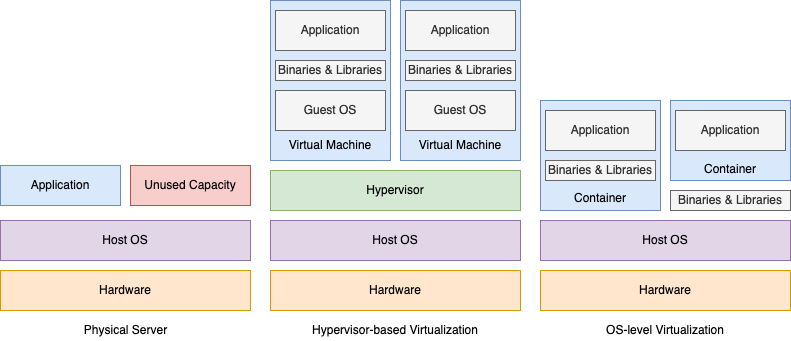
\includegraphics[width=13.5cm]{images/VirtualizationTypes.png}
    \caption{Physical server and two types of virtualization}
    \label{fig:VirtualizationTypes}
  \end{center}
\end{figure}

First of the virtualization technologies, hypervisor-based virtualization adds a hypervisor on top of the host OS and each application instance running is wrapped inside a VM with a dedicated guest OS, binaries, and libraries. This approach is secure and compatible with various host operating systems and processor architectures via hardware emulation. However, the added layers increase the performance overhead significantly. Resources of the server are wasted, especially when multiple VMs are hosted on the same server. In contrast, OS-level virtualization with containers replace the bulky OS with minimal image, such as Alpine. Containers are isolated areas in the host operating system and they do not include an additional guest operating system inside them. Instead, to enable operating system-like functionality, they share parts of the host kernel as well as the host’s libraries and binaries where appropriate. These containers can also include application specific binaries and libraries. \cite{Toimela2017} 

\subsection{Security concerns}

In order to mitigate costs from the application, it is resource-efficient to run multiple instances or different applications in a single server. This applies to companies who own dedicated servers or cloud computing providers with various data center options. These multi-tenant environments may host applications also from untrusted parties. Regardless of the isolation offered by Docker with cgroups and namespaces, the kernel is still shared between the containers. This architectural decision might lead to exposing applications, as it was noticed in 2019 \cite{CVE-2020-14386}\cite{CVE-2019-5736} when attackers could elevate their access to host root. The escaping of container and horizontal traversal via shared kernel creates a security thread of application data integrity.

%You can translate your latex file to rtf with the \texttt{latex2rtf} command in the
%kosh.aalto.fi shell server. Then, the line breaks
%will not be problems for the proofreader of Word.

%Note also that if you have a section or a subsection, you have to have
%at least two of them, or otherwise the section or subsection title is
%unnecessary. Same with the paragraphs: you should not have sections
%with only one paragraph, and single sentence paragraph.

%Aalto library has a comprehensive citation guide ~\cite{bibinstructions}.

\chapter{Kata Containers}
\label{chapter:katacontainers}

The emergence of container technology provides a lightweight operating-system-level virtual hosting environment. Containers profoundly change the development and deployment paradigms of multi-tier distributed services. However, due to the incomplete implementation of system resource isolation mechanisms in the Linux kernel, security concerns still exist for a multi-tenancy container cloud service \cite{Gao2017}. Securing cloud and edge computing services from malicious actors is crucial for companies and MNOs to secure users, services, and data confidentiality and privacy. Kata Containers offers an up-and-coming solution to enhance security with the lightweight isolation layer and compatible integration to the current container orchestration environment. This chapter describes the Kata Containers' architecture, components, and features compared to the current container architecture.

\section{Kata Containers}

Securing container runtime is crucial in MEC to securely operate multiple instances in the same edge node. Compromise of the infrastructure might lead to widespread failures, potentially exposing all user data and risking the confidentiality of the business hosted by the MEC. Meanwhile, low service latency is an essential feature for applications requiring near real-time responses. Slow response times can impair the usability of an edge computing infrastructure. Higher service latencies also result in higher average resource utilization and, therefore, in lower achievable throughput \cite{EverartsdeVelp2020}.

Therefore, multiple solutions have been developed to provide more robust workload isolation using hardware virtualization technology as a second layer of defense. One of the most prominent approaches includes wrapping the container inside a micro-VM during run time. Micro-VM is a lightweight version of traditional VM with reduced overhead stemming from OS, libraries, dedicated resources, and applications in full VM \cite{Flauzac2020}. Micro-VM includes a separate mini kernel to create an isolated environment for the container \cite{Kumar2020}. This dedicated kernel of micro-VM provides isolation of network, I/O, and memory and can utilize hardware-enforced isolation with virtualization extensions. This thesis focuses on Kata Containers as a secure container runtime. Kata Containers perform like containers but provide the workload isolation and security advantages of VMs. Thus, combining the benefits of containers and VMs. \cite{KataContainers}

Kata Containers is open-source software and licensed under the Apache 2.0 license. An Architecture Committee drives long-term development and decisions. Contributors elect the committee's members, who oversee architectural decisions, such as standardization, and resolve technical disagreements between project maintainers. Currently, five members from Apple, Intel, Ant Financial, and Red Hat comprise the committee. \cite{KataContainersGovernance}\cite{KataContainers}

\section{Architecture}

Kata Containers originates from Intel's Clear Containers \cite{ClearContainers} and Hyper runV \cite{runV} in December 2017. The architecture aims to build extremely lightweight VMs that perform like containers but provide the workload isolation and security advantages of adding a virtual machine layer \cite{Randazzo2019}. The design philosophy behind Kata Containers is to integrate seamlessly to the current industry standard of publishing applications as containers. Kata Containers requires no changes to the containers themselves, as the only modification is required on the container orchestrator and the container runtime. Kata Containers integrates into the process of launching and managing the container in the host platform. The main problem Kata Containers is solving is balancing the trade-off between security and speed. In this thesis environment, Kata Containers is deployed within Kubernetes. Figure \ref{fig:KataContainersArchitecture} demonstrates the latest architecture defined version 2.0. This architecture comprises six elements: Kubernetes, container manager, shim, hypervisor, agent, and VM. 

Kubernetes is the container orchestrator and resource manager for automating deployment. Runtime and shim integrate to container manager such as containerd \cite{containerd}. The runtime uses a hypervisor to provide isolation by creating a lightweight VM for each container and then running containerd inside the VM. The Kata Containers introduces a daemon that runs inside the kata-agent VM for managing the containers. This agent uses libcontainer to manage the lifecycle of a container. Kata Containers uses a highly optimized guest kernel to boot the virtual machine, which offers minimal memory usage and fast boot time. This guest kernel provides a better-isolated environment for containers than the traditional security mechanisms of process isolation in containers. \cite{Kumar2020}

Kata Containers, which the OpenStack Foundation stewards, supports industry standards and has been designed along with the OCI \cite{OCI} specifications, thus it supports all the OCI runtime operations \cite{Kumar2020}. As any OCI compliant runtime, the Kata Containers works seamlessly with the Kubernetes Container Runtime Interface (CRI) \cite{CRI}, as well as legacy virtualization technologies, through the container manager such as containerd or CRI-O implementation \cite{Randazzo2019}.

\begin{figure}[ht]
  \begin{center}
    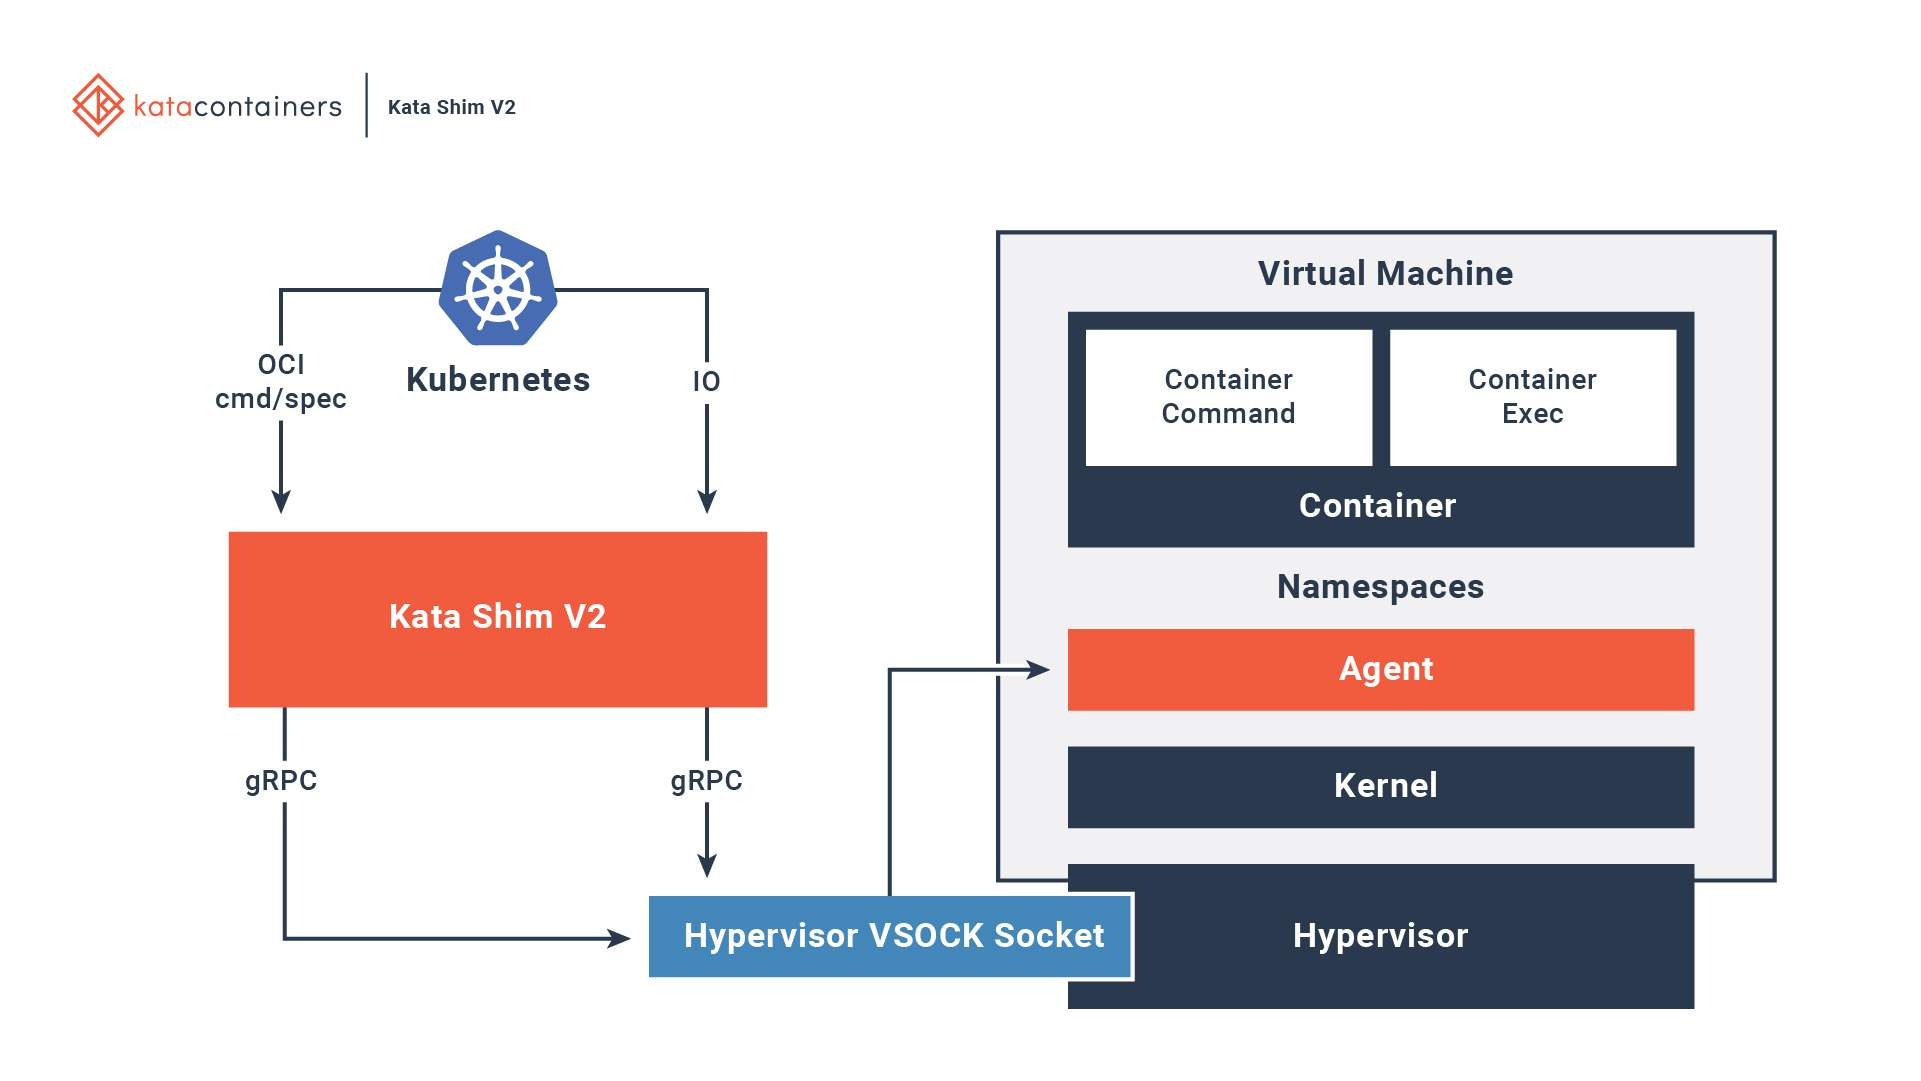
\includegraphics[width=13.5cm]{images/KataContainersArchitecture.jpg}
    \caption{Kata Containers 2.0 architecture \cite{KataContainers}}
    \label{fig:KataContainersArchitecture}
  \end{center}
\end{figure}

\subsection{Kubernetes}

Kubernetes is an open-source container orchestration tool developed by Google, widely used in cloud computing nodes. Kubernetes automates deployment, scaling, and management of containerized applications \cite{Kubernetes}. In addition, Kubernetes monitors the state of containers in the system, and the containers can be automatically re-created in a case of failure \cite{Toimela2017}. Kubernetes offers flexible configuration, and it can be installed inside a VM or on bare-metal. 

Kubernetes launches each container as a pod. Pods are the atomic unit on the Kubernetes platform. A single node can include multiple pods inside it and ties each pod into it within the creation of the pod. Like most distributed computing platforms, a Kubernetes cluster consists of at least one master node and multiple compute nodes. Worker nodes run a node agent kubelet, which communicates with the master node acting as the workload manager. The master node can also act as a worker node, for example, in a single node cluster. Kubernetes uses a Container Networking Interface (CNI)\cite{CNI} component to provide an overlay network for the pods. CNI plugin is responsible for inserting a network interface into the container network namespace and making necessary changes to the host \cite{RedHatCNI}. Each node includes a CNI, such as Calico, Flannel, or Weave.

Each computing node, connected by the CNI plugin, runs a container runtime engine, such as Docker or containerd, along with an agent communicating with the master node. Container runtime is responsible for communicating with the kernel to initiate the containerized process and set up security policies, such as cgroups, SELinux Policy, and App Armor \cite{RedHatCR}. The runtime can be selected on a pod level; thus, a single node can consist of workloads with various runtimes. This flexibility of concurrent runtimes comes in handy whenever non-confidential but highly performance-centric applications need to be deployed in a node within more security-oriented applications. Runtimes are managed by container runtime engines such as containerd and CRI-O.

\subsection{Containerd}

As the Docker project grew, it extracted the container runtime engine into a new project containerd \cite{containerd}. Container runtime engine manages containers inside Kubernetes, including functionality for executing containers, handling low-level storage, and managing container image transfers. Containerd is an open-source implementation of the Kubernetes CRI to enable usage of OCI compatible runtimes. It is an industry-standard container runtime with an emphasis on simplicity, portability, and robustness. It is available as a daemon for Linux and Windows, which can manage the complete container lifecycle of its host system. The flexibility of containerd allows Kubernetes to register and use various OCI-compliant runtimes, such as Kata Containers, as container runtime for running pods. Containerd supports multiple means to download container images, including trust and image verification. Containerd also manages container process lifecycles, low-level storage, and resource isolation as required by the CRI. Containerd launches shim, which further creates the containers. \cite{containerdGithub}

\subsection{Kata Shim V2}

The primary deliverable of the Kata Containers project is a CRI-friendly shim. In the latest version merges the shim, proxy, and runtime into one component. The shim launches Kata-Agent, which launches the container itself. Kata runtime is an OCI compatible container runtime and can handle commands specified by the OCI runtime specification. These commands include invoking the hypervisor for creating a lightweight and fast VM for each container in a pod and launching the Kata Containers instances \cite{Randazzo2019}. The shim enables daemonless containers, allowing the runtime to exit after the container has been launched and then becomes the container's parent. Kata-Agent continues to communicate with other Kata Containers components over RPC protocol \cite{KataContainersArchitecture}. \cite{Crosby}

\subsection{gRPC and ttRPC}

gRPC is a high-performance Remote Procedure Call (RPC) framework that can run in any environment. It connects services in and across data centers with pluggable support for load balancing, tracing, health checking, and authentication. This protocol allows the runtime to send container management commands to the agent. The protocol also to handles the I/O streams such as stdout, stderr, and stdin between the containers. RPC commands manage the container engine, which is containerd in this thesis. Using gRPC via VSOCK interface avoids using previously maintained proxy component as the VSOCK interface can multiplex all gRPC requests \cite{Randazzo2019}. \cite{gRPC}\cite{KataContainersArchitecture}

However, gRPC requires a lot of memory overhead for importing packages and at runtime. While this is great for many services with low-density requirements, this can be a problem when running a large number of services on a single machine or a machine with a small amount of memory. ttRPC is a lightweight protocol gRPC protocol for low-memory environments, such as IoT devices. Apart from the low-memory footprint, ttRPC also offers harnessed security by limiting attack surface and improved observability via metrics about the runtime itself, the VMM, and the guest kernel. Kata Shim V2 offers support also for the ttRPC protocol to communicate with the agent. RPC connection connects Kata Shim V2 with the VMM. \cite{ttRPC}

\subsection{Hypervisor}
\label{subsection:Hypervisor}

VM of Kata Containers instance is launched by VMM, which consists of a Virtual Machine Manager and a hypervisor. The VMM launches Kata-Agent inside the created VM. Kata Containers currently supports four different VMMs: ACRN hypervisor, Cloud Hypervisor, QEMU, and Firecracker. All these VMMs are open-source projects.

ACRN, a reference hypervisor, is built to meet the needs of embedded IoT development. It is developed with low overhead, fast boot-up, and configurations to support various devices and deployment scenarios. ACRN is a type 1 reference hypervisor stack that runs on bare-metal hardware, addressing the gap between data center hypervisors and hard partitioning hypervisors. \cite{ACRN}

Cloud Hypervisor is a VMM that runs on top of the Kernel-based Virtual Machine (KVM). The project focuses on exclusively running modern cloud workloads on top of a limited set of hardware architectures and platforms. Customers inside a cloud provider usually run cloud workloads, and most I/O operations are handled by performant para-virtualized devices, such as Virtio. \cite{CloudHypervisor}

QEMU is a generic machine, userspace emulator, and virtualizer. QEMU is capable of emulating a complete machine in software without any need for hardware virtualization support. It can also integrate with the Xen and KVM hypervisors to provide emulated hardware while allowing the hypervisor to manage the CPU. Kata Containers uses a special version of QEMU name qemu-lite to improve boot time and reduce memory footprint with features such as machine accelerators, kernel same-page merging, hot plug devices, and Fast Template \cite{Randazzo2019}. \cite{QEMUGithub}\cite{QEMU}

Machine accelerators are architecture-specific for improving performance. One of these enables direct access storage, allowing sharing the host rootfs in read-only mode to a persistent memory device to the VMs. Kernel same-page merging is a KVM feature that allows sharing identical memory pages amongst different VMs. This sharing deduplicates memory to maximize container density on a host. Hot-plug devices allow VMs to start with minimum resources for faster boot time and a tiny memory footprint. The hypervisor allocates the VM more resources as soon as requested by hot-plugging devices on the fly. Fast Template is a pool of pre-configured lightweight VMs ready to deploy quickly. The featured QEMU hypervisor is also available with VirtioFS support, which is a shared file system that lets virtual machines access a directory tree on the host, accelerating I/O performance in some context \cite{virtio-fs}. \cite{Randazzo2019}

Firecracker is a community-driven VMM, backed and originally developed by AWS. Firecracker uses KVM to launch workload in lightweight micro virtual machines. Of Amazon's cloud products, Firecracker is deployed at least in AWS Lambda and Fargate. Firecracker currently supports Intel CPUs, with AMD and Arm support in developer preview. \cite{AWS}\cite{FirecrackerDesign}\cite{Debab2021}

\subsection{Agent}

Agent, also known as Kata-Agent, launched by the VMM, resides inside the Kubernetes pod in the computing node, and its main task is to spawn the container process. The agent sets up the environment for managing containers and processes running within those containers. The agent process runs as a daemon inside the virtual machine. This agent runs a ttRPC or gRPC server in the guest using a Virtio serial or VSOCK interface, which the VMM exposes as a socket file on the host. \cite{KataContainersArchitecture}

\subsection{Container}

Kata Containers architecture isolates a container by wrapping it inside a micro-VM with a dedicated kernel. This extra layer provides isolation of the network by minimizing container escapes of a malicious actor. I/O and memory can utilize hardware-enforced isolation with virtualization VT extensions. Wrapping the container inside a micro-VM possible adds an overhead to performance, which is discussed more in Chapter \ref{chapter:evaluation}. \cite{KataContainers}

Kata Containers is OCI compliant; thus, the same standard shared by Docker containers guarantees compatibility. However, for now, only Linux operating systems and container images are supported in host and guest.

\section{Features}

The architecture and components of Kata Containers allow a different approach to hosting containers in the environment compared to Docker runtime. The most crucial feature of Kata Containers is the extra layer of isolation provided by the micro-VM. Due to this isolation layer, some changes are needed to the network layer to allow OCI compatible networking for the container runtime engine, further discussed in this section. The support for the most crucial Far Edge Cloud features is discussed in Chapter \ref{chapter:evaluation}. The inclusion of a micro-VM adds a layer of isolation but introduces a new challenge for the containerized environment with resource allocation.

\subsection{Isolation and resource allocation}

Kata Containers are created on top of traditional namespace containers. The hardware virtualization interface is the basis of this additional layer. Kata Containers launches a lightweight virtual machine and uses the guest's Linux kernel to create a container workload. In Kubernetes and the Kata implementation, the sandbox is carried out at the pod level. A virtual machine such as KVM creates the sandbox for workload isolation \cite{KataContainersVirtualization}. Because KVM is a hypervisor emulating complete hardware and hosts another Linux kernel inside, it is considered even harder to escape this environment resulting in harnessed security \cite{Eder2016}.

Kubernetes environment deploys application containers inside a pod. Upon creating a pod, it requests resources, which most commonly are CPU, memory, and huge pages, defined in the configurations. The allocated resources are reserved for the application running. Traditionally the resources allocated are a slice from the resource described in Figure \ref{fig:KataContainersStack}. Kata Containers environment virtualizes the hardware for the guest kernel, likewise in hypervisor-based virtualization described in Figure \ref{fig:VirtualizationTypes}. Resource allocation increases security by dedicating specific cores for a VM but might decrease the overall performance. Due to the nature of VMs, Kata Containers is unable to allocate resources dynamically without VM restart. In contrast, Kubernetes allows containers to set lower and upper limits for CPU and memory resources, which are requests and limits \cite{KubernetesContainerResource}. The VM architecture changes the way Kata Containers CNI is connected with the host networking, as discussed in the next section.

\begin{figure}[ht]
  \begin{center}
    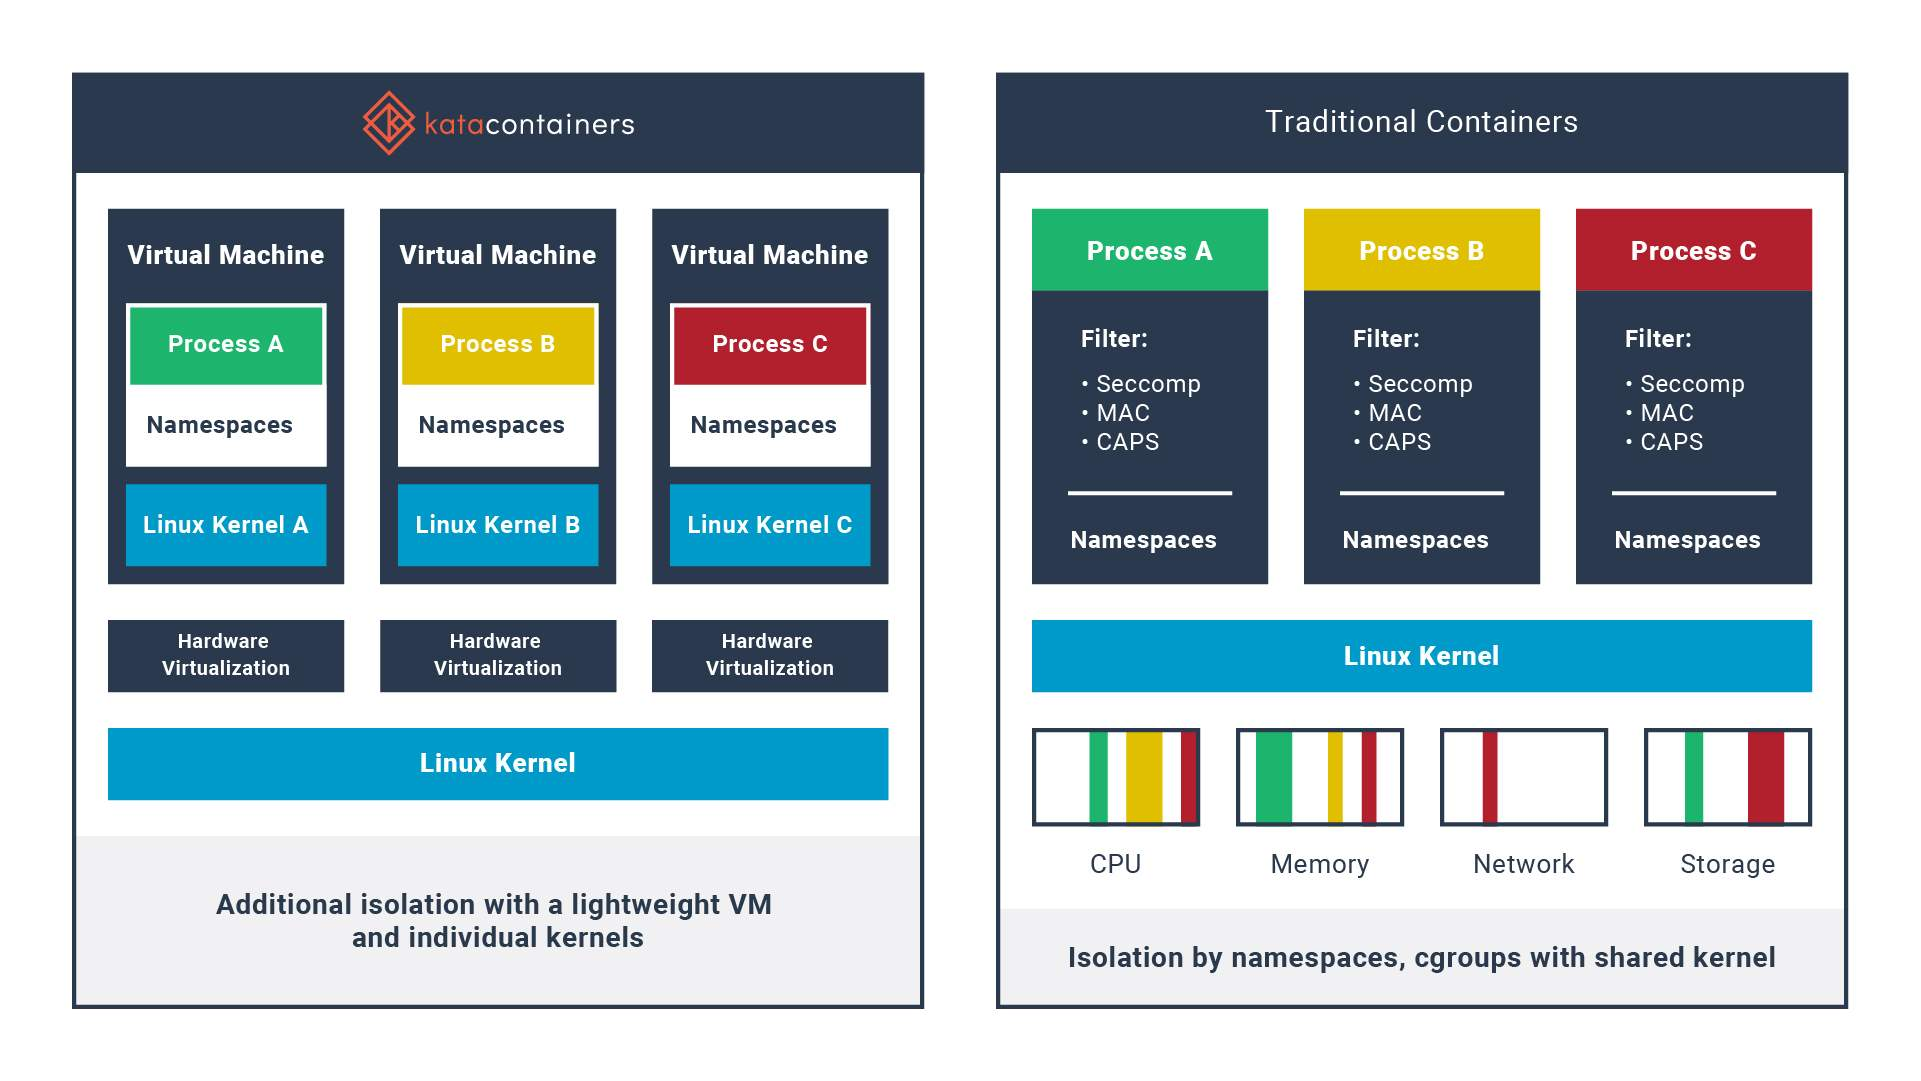
\includegraphics[width=13.5cm]{images/KataContainersStack.jpg}
    \caption{Kata Containers and traditional container stack \cite{KataContainers}}
    \label{fig:KataContainersStack}
  \end{center}
\end{figure} 

\subsection{Networking}

Traditionally container engines, such as Docker, add one end of a virtual ethernet pair into the container networking namespace. The other end of the pair is added to the host networking namespace. However, many VMMs cannot handle virtual ethernet interfaces. Typically, TAP interfaces are created for VM connectivity. As described in Figure \ref{fig:KataContainersNetwork} Kata runtime overcomes the incompatibility between typical container engine's expectations and virtual machines by connecting virtual ethernet interfaces to kernel virtual network device TAP using Traffic Control. TAP works on data link layer carrying ethernet frames and is often used to create a userspace network bridge. \cite{KataContainersArchitecture}

Kata Containers supports both Container Network Models adopted by Docker and CNI adopted by Kubernetes and Podman. Both models provide the freedom of selection for a specific type of container networking, join one or more networks, and use multiple network drivers concurrently \cite{Randazzo2019}. In addition, Kata Containers supports both IPv4 and IPv6 networks.

\begin{figure}[ht]
  \begin{center}
    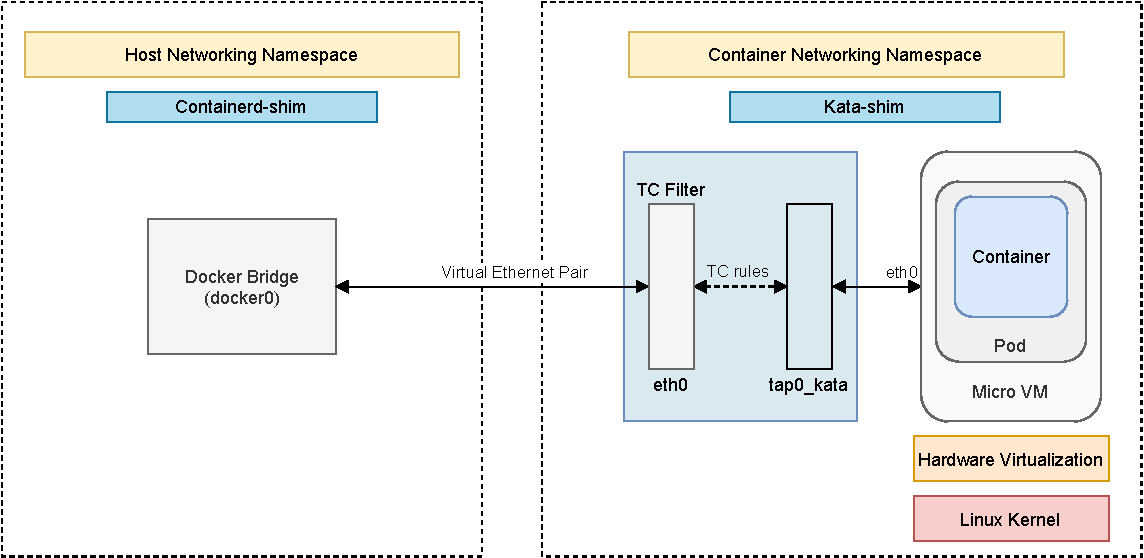
\includegraphics[width=13.5cm]{images/KataContainersNetwork.pdf}
    \caption{Kata Containers network overview \cite{KataContainersArchitecture}}
    \label{fig:KataContainersNetwork}
  \end{center}
\end{figure}

\subsection{Storage}

Kata Containers can manage the storage both at the file system level and at the block level. At the file system level, virtualized environment shares container workloads through VirtioFS. This shared file system permits VMs to access a directory tree on the host. Kata Containers uses VirtioFS to share container volumes, secrets, config-maps, configuration files, and the container rootfs on the host with the guest VM. VirtioFS provides significant performance and POSIX compliance improvements compared to 9pfs, supported in Kata Containers. VirtioFS was started at Red Hat and developed in the Linux, QEMU, FUSE, and Kata Containers open-source communities. \cite{virtio-fs-Kata}\cite{virtio-fs}

Kata Containers can hot-plug and remove block devices, a data storage device that supports reading and optionally writing data in fixed-size blocks, sectors, or clusters. This support for hot-plugging makes it possible to add new block devices for containers started after launching the VM without a reboot. Hot-plugging adds flexibility and improves the uptime of services. Regardless of general support for hot-plugging and various file systems, its exact compatibility might vary depending on the VMM and hypervisor. \cite{KataContainersArchitecture}\cite{KataContainersVirtualization}

\section{Summary}

Kata Containers offers a potential solution for lightweight workload isolation compatible with current Kubernetes and container environments, harnessing the benefits of container orchestration. Kata Containers' architecture includes several components differing from the current defacto standard. Regardless of this difference, the basic functionalities such as block and filesystem storage and Docker-like networking interface are offered to support OCI standards. One significant difference between Kata Containers and the OS-level virtualization, such as Docker or Kubernetes with runC as the container runtime, is the lack of dynamic resource allocation on a shared infrastructure. This is a compromise between security and resource usage efficiency. The next chapter discusses more the implementation of Kata Containers in the Far Edge Cloud environment.
 
\chapter{Kata Containers in Far Edge Cloud}
\label{chapter:implementation}

Telco systems are a complex environment with multiple requirements for connectivity and performance. This chapter discusses the requirements of telco systems, implementation, and possible limitations of Kata Containers in this environment. The performance and tests are described in Chapter \ref{chapter:evaluation}. The features discussed in this chapter are related to Kubernetes, the container orchestrator, configurations.

\section{CPU}

Telecommunication applications are computing heavy, which require efficient usage of resources. One of the requirements telco applications have for infrastructure is the support for core isolation. This feature allows dedicating a single core to a process in order to minimize interruptions for the process. Core isolation involves removing all user-space threads, unbound kernel threads, and blocks interruptions from the system \cite{CPUisolation}. The benefit of a dedicated core for a process is enhanced performance and extended use of CPU caches.

The core isolation is accomplished with a specific Kubernetes plugin, such as Intel CMK\cite{IntelCMK} or Nokia CPU Pooler\cite{NokiaCPUPooler}. These plugins manage predefined physically separated pools of resources between applications. CPU Pooler supports two explicit types of CPU pools; exclusive and shared. Kubernetes allocates resources to a container on container creation. If the container has not requested specific resources from these pools, it will be assigned to a third, named default, pool. The exclusive pool allows applications for uninterrupted resources and is preferred for latency-sensitive workloads.

Kata Containers the architecture includes a Kata-agent and a guest kernel for each pod as described in Figure \ref{fig:KataContainersComponents}. These resources need to be assigned to a second core, a shared resource between other pods, or a core of the exclusive pool. The shared resources, defined by shared and default pools, can also host general cluster components such as monitoring and DNS.

\section{Memory}

Modern telco systems rely on high-throughput and low-latency data sharing between containers within pods. Writing and reading a shared block of memory between containers offers the fastest way for shared information. In Kubernetes, containers can share IPC namespaces inside a pod with the help of pod security policies \cite{PodSecurityPolicyKubernetes}. Configuration of these policies enables usage of HostIPC, which controls whether the pod containers can share host IPC namespace.

Kubernetes manages memory in blocks known as pages. In most systems, the default page size is 4 kilobytes; consequently, 1 megabyte of memory equals 256 pages. CPUs have a built-in memory management unit managing a list of these pages on hardware. This management unit, Translation Lookaside Buffer (TLB), has a fixed number of pages it can store. Once the number of pages exceeds the number defined in TLB, the system falls back to a slower, software-based address translation. This transition results in degraded performance. Since the number of pages TLB stores is fixed, the only way to decrease TLB miss is to increase the page size with huge pages. \cite{HugePagesOpenShift}

Huge pages is a memory page with a size larger than 4 kilobytes. In x86\_64 architectures, the two popular sizes are 2MB and 1GB. In order to use huge pages, the application must support the use the larger page sizes. The high-performance telco applications use huge pages; therefore, huge pages are crucial to maintaining performance.

Kubernetes supports the allocation and consumption of pre-allocated huge pages by applications in a pod \cite{HugePagesKubernetes}. Kata Containers also support using huge pages; however, it needs configuring explicitly in a custom Kata Containers kernel. As Kata Containers architecture consumes more memory than a native design with runC, the pod must be allocated enough resources to support huge pages.

\section{Storage}

High-performance Kubernetes storage options are usually limited to storage locating close to the computing unit. Thus, network storages or block storages hosted on a commercial cloud, which relies on data transmission via a network, are insufficient. Telco systems use three types of storage for high-performance applications: emptyDir, hostPath, and local. EmptyDir is a non-persistent volume, implying it does not retain data stored if the attached pod is removed from a node. In contrast, hostPath and local storages are Persistent Volumes (PV), a Storage Class type defined in Kubernetes. These storages are individuals of restructuring the cluster architecture and thus are applicable for storing user-related data or logs. In contrast, emptyDir is mainly used for session-specific data or offloading memory temporarily.

\subsection{emptyDir}

Kubernetes creates emptyDir volume during pod assignment to a node and lives as long as the pod runs on that node. emptyDir volume is initially empty. All containers in the pod of the emptyDir can read and write the files in the volume. Some use cases for emptyDir are scratch space during disk-based merge sort, checkpointing during a long computation in case of crashes, and holding files that a content-manager container fetches while a webserver container serves the data. \cite{VolumesKubernetes}

Various storage mediums such as disk or SSD can back emptyDir volumes. However, emptyDir also supports RAM-backed filesystem tmpfs, which offers a high-speed alternative to harddrive-based volumes. The system clears the tmpfs filesystem on node reboot, and any data written on it counts against the container's memory limit. \cite{VolumesKubernetes}

\subsection{Persistent Volume}

Persistent Volume (PV) is a storage piece in the cluster, providing storage having a lifecycle independent of any individual pod using the PV. It is provisioned dynamically or by an administrator. Kubernetes supports filesystem and block-based persistent storage resources, such as Network Filesystem (NFS), SCSI over IP (iSCSI), local storage devices, or AWS Elastic Block Store \cite{AmazonEBS}.\cite{PV}

PVs can be mounted to nodes in Kubernetes with three different access modes: ReadWriteOnce, ReadOnlyMany, and ReadWriteMany. ReadWriteOnce allows only one node for read and write operations. ReadOnlyMany is a read-only mode allowing multiple nodes for simultaneous access. In contrast, ReadWriteMany allows multiple nodes for simultaneous read and write operations. Based on the type of PV, the support for access modes varies. In this Thesis, we will focus on two high-performing PV options, which are hostPath and local. \cite{PV} 

A hostPath volume mounts a file or directory from the host node's filesystem into the pod. Some use cases for hostPath include running a container that needs access to Docker internals or running cAdvisor in a container that requires access to the system directory. HostPath is only applicable inside a single node; however, multiple pods can write simultaneously into the same file or directory.

Local volume represents a mounted local storage device such as a disk, partition, or directory \cite{VolumesKubernetes}. Local volumes can only be created statically, and dynamic provisioning is not supported. Compared to hostPath volumes, local volumes are used in a durable and portable manner without manually scheduling pods to nodes. Local volumes are subject to the availability of the underlying node. Downtime of the node disables all access to the storage attached, regardless of the state of the storage container. This failure reduces the availability of the storage and possibly causes potential data loss.

The node mounts a local volume as a filesystem or raw block device. These raw block volumes are mounted into a pod without any filesystems on it. The filesystem layer introduces unneeded overhead, which slows down the I/O process. Some specialized and high-performance applications require direct access to a block device to maximize performance. An everyday use case is databases, which prefer to organize their data directly on the underlying storage. Raw block devices are also commonly used by software that implements its storage service. \cite{RawBlockKubernetes}

\section{Network}

Kubernetes networking supports a feature for sharing process namespaces between containers in a pod. When process namespace sharing is enabled, processes in a container are visible to other containers in that pod. This feature is handy for configuring cooperating containers, such as log handler sidecar containers, or troubleshooting container images that do not include debugging utilities like a shell. Process Namespace Sharing is disabled by default and needs to be enabled in the pod configuration in Kubernetes. This feature also enables signaling processes in other containers. For example, SIGHUP can be sent to Nginx to restart the worker process allowing more flexible container operation in the node. \cite{ShareProcessNamespaceKubernetes}

Telco systems use shared network namespaces for interprocess communication through shared memory and Unix sockets. This communication is vital for multiprocess applications, where each process handles a specific part of the business logic and needs to communicate with each other. In a telco environment, low latency for operations needs to be guaranteed. Therefore the latency requirement is not satisfied using network-based communication such as through IP. Kata Container supports process namespace sharing in the latest versions.

\subsection{Multus}

Telco networking requires connecting to multiple networks simultaneously. By default, Kubernetes supports only a single network, apart from loopback, attached to a pod. In order to extend the network interface, Kubernetes has adopted the Multus CNI plugin to the cluster stack.

Multus CNI \cite{Multus} is a container network interface plugin for Kubernetes that enables attaching multiple network interfaces to pods. By default, in Kubernetes, each pod has one network interface. With the help of Multus, pods can be multi-homed and attached with multiple interfaces. Figure \ref{fig:Multus} demonstrates a Multus enabled pod setup with two networks in Kubernetes. The pod includes three interfaces: net0, net1, and eth0. Network attachments net0 and net1 connect to outbound services using CNI plugins such as vlan, vxlan, or ptp. eth0 interface connects to Kubernetes cluster network to connect with the server or services such as kubernetes-api-server or kubelet. Enabling Multus for the Kata Containers environment is supported and requires no extra configuration apart from the Kubernetes configuration. \cite{MultusUbuntu}

\begin{figure}[ht]
  \begin{center}
    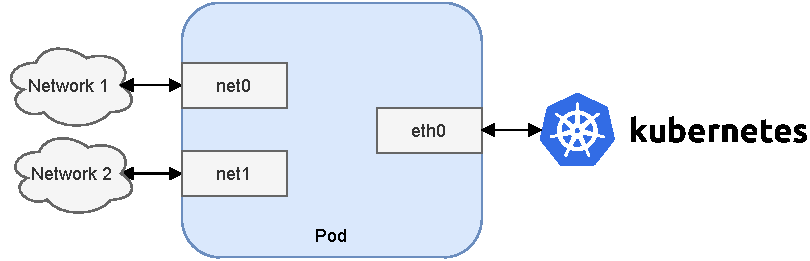
\includegraphics[width=13.5cm]{images/Multus.pdf}
    \caption{Multus enabled pod with two networks}
    \label{fig:Multus}
  \end{center}
\end{figure}

\subsection{SR-IOV}
\label{section:SR-IOV}

I/O throughput is critical to high-performance telco systems. I/O intensive servers may waste CPU cycles waiting for I/O data or spinning on idle cycles, reducing system performance by increasing latency. Single Root I/O Virtualization (SR-IOV) standard allows an I/O device, such as a network interface controller (NIC), to be shared by multiple VMs. The SR-IOV technology is a hardware-based virtualization solution that improves both performance and scalability. \cite{Dong2012}

Traditionally, when a guest accesses the I/O device, VMM needs to intervene in the data processing to share the physical device. The VMM intervention leads to additional I/O overhead for a guest OS. SR-IOV provides hardware enhancements for the Peripheral Component Interconnect Express (PCIe) device, which aims to remove major VMM interventions for performance data movements, such as the packet classification and address translation. An SR-IOV-capable device can create multiple lightweight PCI function entities, known as Virtual Functions (VF). Each VF can be assigned to a VM for direct access but still shares major device resources, achieving both resource sharing and high performance. \cite{Dong2012}

In Kubernetes, Kata Containers supports SR-IOV with a CNI plugin \cite{SR-IOVOpenShift} as visualized in Figure \ref{fig:SR-IOVNode}. Additionally, the Kata runtime detects virtual functions in the container's network namespace to use SR-IOV for network-based devices. In order to enable SR-IOV with Kata, the user needs to install a specific Docker plugin. The created network is based on a physical function device. \cite{SR-IOVKataContainers}

\begin{figure}[ht]
  \begin{center}
    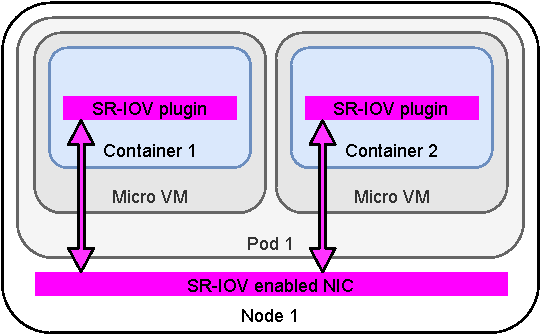
\includegraphics[width=13.5cm]{images/SR-IOVNode.pdf}
    \caption{SR-IOV enabled node with two containers in a single pod}
    \label{fig:SR-IOVNode}
  \end{center}
\end{figure}

In order to set up a host for SR-IOV, the system needs to support Intel Virtualization Technology for Directed I/O (VT-d), and the NIC device needs to support SR-IOV. Also, the host kernel must have Input-Output Memory Management Unit (IOMMU) and Virtual Function I/O (VFIO) support.

\subsection{Hardware acceleration}

Hardware acceleration is the use of hardware specifically crafted to perform functions more efficiently than software running on general-purpose CPUs. The hardware-accelerated process can highly enhance the performance of cloud workloads by increasing throughput and decreasing latency and energy consumption. Hardware acceleration can be used of GPUs for computing, SmartNIC \cite{SmartNICIntel}, or purpose-built application-specific integrated circuit (ASIC) such as System on a Chip (SoC).

The main use of hardware acceleration for edge cloud environment is computing offloading to GPUs, which performs specific workloads faster and frees CPU cycles for other tasks, thus improving throughput. Kata Containers supports passing certain GPU resources from the host into the container using GPU passthrough and GPU mediated passthrough. GPU passthrough, such as Intel GVT-d, allows direct assignment of an entire GPU to a single user, passing the native driver capabilities through the hypervisor without any limitations. Mediated GPU passthrough, such as Intel GVT-g with multiple VMs to one physical GPU, is a full GPU virtualization solution with mediated passthrough. A virtual GPU instance is maintained for each VM, with part of performance-critical resources directly assigned. The ability to run a native graphics driver inside a VM without hypervisor intervention in performance-critical paths achieves a good balance among performance, feature, and sharing capability. \cite{GPUKataContainers}

Plugins such as vAccel \cite{vAccel} offer QEMU and Firecracker VMM support for hardware acceleration for serverless computing. The focus of vAccel is to provide true device sharing in the shared cloud and edge infrastructure with portability and modular design.
		
\section{Logging}

In a containerized environment, containers should not store any persistent data. Therefore, logs should not be stored inside the container. Otherwise, a failure in the container would also destroy the logs \cite{Toimela2017}. However, logging to a location on the host via a persistent volume or hostPath is a viable option to store the logs in a safe and accessible way. 

However, if the kernel is shared between the pods, it adds an extra point of failure for the environment. A kernel panic or dump might render the whole environment useless until a reset. Kata Containers provides the workload with the guest kernel. Therefore, the host uses a dedicated kernel that enhances robustness and allows easier debugging in the cluster.

\section{Summary}

Kata Containers fits well to the telco environments, significantly strengthening the FEC infrastructure's security features. The architecture of Kata Containers supports the most crucial requirements of FEC, such as CPU isolation, huge pages, Multus, SR-IOV, and hardware acceleration natively or with third-party plugins. In addition to these features, the architecture allows more robust logging and debugging functionalities of the containers. However, these architectural difference of Kata Containers in comparison to native Docker environment affects the performance and resource efficiency which are evaluated in the next chapter.


\chapter{Evaluation}
\label{chapter:evaluation}

Kata Containers hardens the security of containerized environment by adding the extra layer of security with the micro-VM. The architectural change and new components of the environment enable the additional security features. However, these components, such as the micro-VM and hypervisor, come with a possible price of degraded performance and computational overhead. Previous work, such as \cite{EverartsdeVelp2020} and \cite{Kumar2020} have examined the performance when compared Kata Containers against the native runtime runC, the most common OCI-compliant runtime. In these two papers, Kata Containers architecture design results in a performance decrease in I/O throughput and overhead in memory and CPU utilization. However, the results in these papers are highly dependant on the underlying test environment. Furthermore, these tests do not consider the latest development and performance optimization of Kata Containers' performance. This paper evaluates the system performance in an environment simulating a telco Edge Cloud architecture and regular workload.

\section{Test architecture}
\label{section:test_architecture}

Telco applications are relying on high-performing and optimized computing. The ever-more increasing performance requirements from users add a great demand on the underlying infrastructure. Software and hardware-based architectural changes to the Edge Cloud environment need to be carefully evaluated before implementing them into the production. Otherwise, it might stall the performance and significantly decrease the performance for mobile network users.

The test environment, visualized in Figure \ref{fig:TestArchitectureCluster}, is a simple single-node cluster with one container. The main focus of the tests is to evaluate the impact of Kata Containers and the choice of the hypervisor to I/O operations throughput and latency on various storage methods, such as PV, emptyDir, and hostPath. Table \ref{table:TestMatrix} describes the full test combination matrix. The test cluster is hosted on K3s \cite{K3s} version 1.17.3, a lightweight version of Kubernetes supporting the identical API. K3s is Kubernetes distribution built for IoT and edge computing with a lower footprint on memory and disk usage. K3s uses containerd as a native container runtime engine. Due to compatibility issues, Kata Containers uses version 1.12.0, which benefits from the simplified Kata Shim V2 \cite{KataContainersArchitecture} architecture described in Figure \ref{fig:KataContainersArchitecture}.

\begin{figure}[ht]
  \begin{center}
    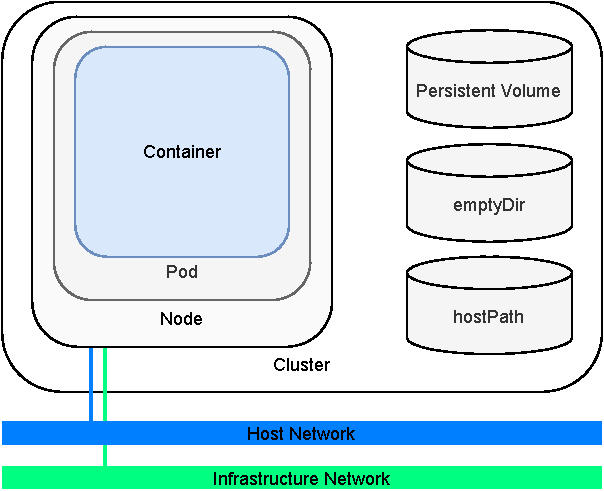
\includegraphics[width=12cm]{images/TestArchitectureClusterSimple.pdf}
    \caption{Kubernetes test cluster overview}
    \label{fig:TestArchitectureCluster}
  \end{center}
\end{figure}

\section{Methodology}

The tests of this thesis aim to measure the possible performance degradation of I/O operations, such as bandwidth and completion latency. A dedicated server hosts the test environment, and the underlying hardware is built and tailored to support Edge and Far Edge Cloud deployments. The server includes an Intel Xeon 6212U CPU with 24 cores and 48 threads with x86 architecture at 2.40 GHz clock-speed and 192 GB of DDR4 memory at 2933 MHz clock speed, which is shared to the cluster.

The host runs CentOS 8 and uses Linux kernel version 4.18.0-240.22.1, affecting mostly bare-metal and runC environments. In Kata Containers, CLH and QEMU with VirtioFS use version 5.6.0, whereas QEMU uses a slightly older kernel version of 5.4.60. The difference in kernel versions might affect the performance results due to optimization in resource usage and I/O operations. The server uses Intel's SSD \cite{IntelSSD} for disk-based I/O operations. This disk's theoretical maximum bandwidth for sequential read operations is up to 560 MB/s and 510 MB/s for write operations.

The performance tests run with Fio \cite{FIO}, an I/O performance tester intending to simulate a variety of I/O workloads without resorting to writing tailored test cases repeatedly. Fio supports various test configurations such as multiple threads, block sizes, I/O sizes, and I/O patterns. In this thesis, the tests are time-based, where each test runs for 30 seconds. The file size of each writable file is 2 GB. The Fio configuration file, also known as the job file, is described in Appendix \ref{appendix:fio_jobfile}. Each test is repeated three times, and averaging the results. Table \ref{table:TestMatrix} describes the test combination matrix. In the tests, each possible combination is sampled, resulting in 1428 different test scenarios. To be noted, bare-metal tests allow only I/O to a disk volume. Kubernetes hosted tests, runC and Kata Containers, leverage all disk and memory-based volumes. The span of the disk for bare-metal volume is the full 480 GB, whereas Kubernetes hosted volumes can be split into smaller units, resulting in a narrower span for read and write operations. This variance in span highly affects the efficiency of seek operations.

\begin{table}[ht]
\centering
\caption{Test combinations matrix}
\vspace{\baselineskip}
\begin{tabular}{| c | c | c | c | c |}
\hline
\textbf{Runtime} & \textbf{Jobs} & \textbf{Block size} & \textbf{I/O pattern} & \textbf{I/O device} \\ 
\hline
Bare-metal & 1 & 512 & read & emptyDir (memory) \\
\hline
runC & 2 & 1024 & write & emptyDir (disk) \\ 
\hline
CLH & 3 & 2048 & randread & local (PV) \\
\hline
QEMU & & 4096 & randwrite & hostPath \\
\hline
QEMU VirtioFS & & 8192 & & \\
\hline
& & 32768 & & \\
\hline
& & 65536 & & \\
\hline
\end{tabular}
\label{table:TestMatrix}
\end{table}

The test matrix consists of five columns: runtime, jobs, block size, I/O pattern, and I/O device, the runtime of the tests refers to the container runtime or hypervisor. In the case of bare-metal, the test is run directly on the host without containerization. In bare-metal test runs, the performance test is launched with CPU affinity to an isolated CPU with taskset \cite{taskset} command. Jobs refer to the number of concurrent clones. Each clone of the job is spawned as an independent thread or process. Block size is the size in bytes for I/O units applying for reads and writes. I/O pattern has sequential and random pattern reads and writes. I/O type of the test is buffered, as configured in the Fio job file. I/O device refers to the storage volumes used for the test destination. EmptyDir is created within the container of these storage volumes, whereas the host maintains local Persistent Volume and hostPath.

Fio test suite is wrapped inside a Docker image with a Linux OS Alpine \cite{Alpine}, which aims to deliver general-purpose Linux with security, simplicity, and resource efficiency. The tests containers are deployed into the test cluster with Helm \cite{Helm}, a package manager for Kubernetes helping with the deployment of applications. These applications are deployed in Kubernetes pods as Guaranteed Quality-of-Service \cite{QOSKubernetes} with two CPUs and 18 GB of memory to support the tests. However, each Kata Containers' VM and runC container gets assigned only with one CPU. This restriction allows better comparison tests to bare-metal tests run on an isolated single CPU environment. The Guaranteed Quality-of-Service prevents Kubernetes from scheduling other containers for the same core. However, this does not guarantee that the underlying system would not assign low-level system tasks on the same core. The comparable isolation to taskset, as in bare-metal, could only be achieved with core isolation plugins, such as Nokia's CPU Pooler, limiting the absolute comparison of results described in the next section.

\section{Results}

Previous work \cite{EverartsdeVelp2020}\cite{Kumar2020}\cite{StackHPCKata}\cite{Randazzo2019} on measuring Kata Containers' performance resulted in highly unified performance between bare-metal and runC. In read and write tests, runC slightly outperformed the tested Kata Containers setups with faster throughput and lower resource usage. However, the results of these papers varied due to the diversity in underlying infrastructure and the difference in test frameworks. None of these researches tested the whole spectrum of hypervisors and various storage options offered in the Kubernetes environment.

The hypervisor of Kata Containers adds its resource and latency overhead to the performance. The focal point of I/O tests is to evaluate the performance of Kata Containers with various hypervisors against the runC runtime and determine the inherent performance metrics of each hypervisor and evaluate storage volume performance. As described in Table \ref{table:TestMatrix}, the test includes three different Kata Containers' hypervisors: CLH, QEMU, and QEMU with VirtioFS. Secure container runtimes leveraging micro-VM include hypervisor to the stack. This hypervisor includes its cache, giving a false impression of superior performance compared to bare-metal and runC. The caching feature restricts the possible comparison of bare-metal's and runC's performance evaluation to secure runtimes in read operations for all disk-based storage volumes.

Kubernetes offers multiple storage options for various deployments, and each of these options provides slightly different performance and features. The tests include four storage options suitable for the telco environment: disk and memory-based emptyDir, hostPath as Persistent Volume, and hostPath. The second key point of the tests is to evaluate these storage methods concerning block sizes between 512 bytes and 64 KBs and concurrent jobs from one to three. It is essential to make the distinction of evaluating the best option for non-persistent and persistent volumes.

Tests to evaluate the performance are run individually to minimize interference, and the final results are averaged out of three test runs. Fio test suite provides a comprehensive catalog of parameters as test results. These test results are divided into two categories, which are bandwidth and completion latency. Bandwidth, or I/O throughput in megabytes per second, is the sum of block size multiplied by the number of I/O operations per second. Bare-metal test results work as a benchmark of the best-case scenario for disk-based volumes. Completion latency describes the completion time in milliseconds for key percentiles such as 50\% and 99\%. 

\subsection{Bandwidth}

Figure \ref{fig:ResultsVolumeByRTC4096-1} visualizes the effect of runtime class for reading or write bandwidth for the four storage volumes. Bare-metal is not comparable with memory-based emptyDir, due to significantly different techniques used, and thus it is not plotted for emptyDir on memory. Memory-based emptyDir achieves the highest bandwidth as it reaches over 2 GB/s with sequential read and over 1.9 GB/s with sequential write for all runtimes. The performance slightly degrades for random pattern read and write operations but achieves over 1.5 GB/s performance for all runtimes. Hypervisor-based runtimes seem to perform highly alike, with only minor differences between them. Based on the acquired test results in Figure \ref{fig:ResultsPVByBS-1} with PV as volume and one concurrent job, CLH outperforms QEMU-based runtime classes in tests with smaller block sizes, 512 to 8192. The trends flip for tests with block sizes 32768 and 65536. Due to the caching, bare-metal and runC are not comparable against Kata Container runtimes in reading operations.

Hypervisor caching affects the confidence in the test results highly for reading operations, especially random pattern read. When fetching data from a storage volume, the system first checks the memory-based cache for the request data. If it is found, the seek on a storage volume is skipped. As the size of each job file in Fio was relatively small, the hit probability of the requested block being cache is high, which skews the results in favor of Kata Containers runtimes. This effect of caching is visible in Figure \ref{fig:ResultsVolumeByRTC4096-1} where Kata Containers runtimes outperform bare-metal and runC in all disk-based sequential, and random pattern read tests by a clear margin. The same skew is also visible in Figure \ref{fig:ResultsHPClatByRTC4096-2}, where completion latency is lower for hostPath read operations.

\begin{figure}[ht]
  \begin{center}
    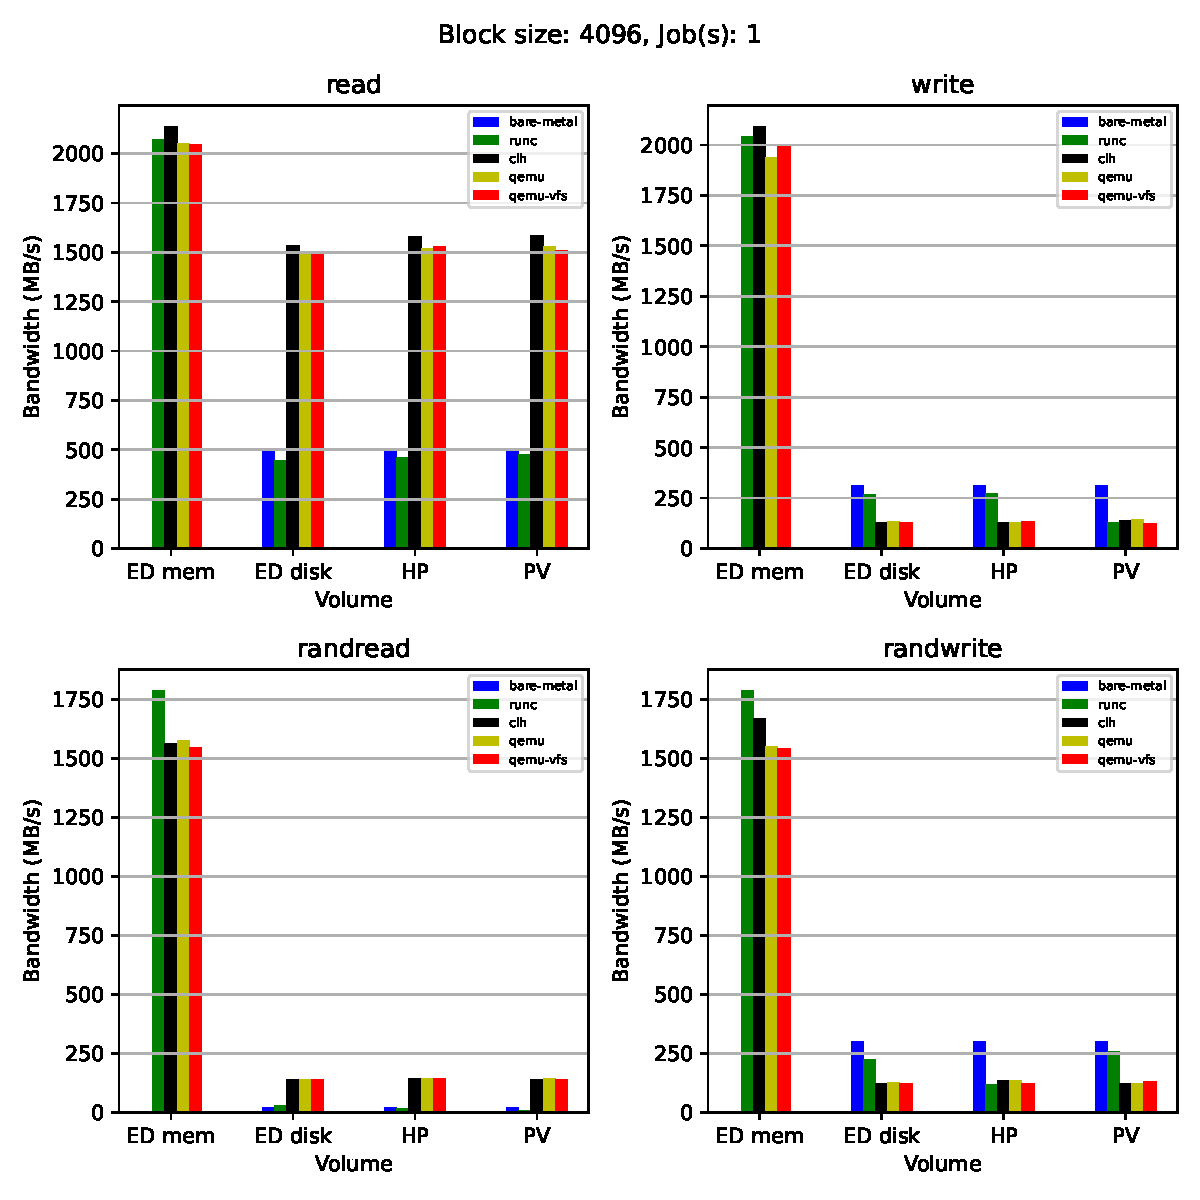
\includegraphics[width=12cm]{results/subplot_bw_by_volume_with_bare(4096,1).pdf}
    \caption{Comparison of volume performance by runtime classes for 4096 bytes block size and one job}
    \label{fig:ResultsVolumeByRTC4096-1}
  \end{center}
\end{figure}

For write operations in Figure \ref{fig:ResultsVolumeByRTC4096-1}, runC averages 224 MB/s on sequential and 201 MB/s on random patterns with disk-based volumes. In contrast, Kata Containers averages 131-135 MB/s on sequential and 127-129 MB/s on random pattern write operations. The proportional drop in performance is significant, resulting in around 36-40\% drop in the bandwidth. This drop in performance is radical compared to memory-based emptyDir, which suggests leveraging memory for as much as possible. Kata Containers runtimes perform on the same level, with no clear differences in the bandwidth across them. The performance of disk-based volumes is highly correlated, with no difference in performance for persistent and non-persistent volumes for Kata Containers runtimes.
    
Figure \ref{fig:ResultsPVByBS-1} visualizes the effect of block size on the bandwidth on Persistent Volume. The caching affects Kata Containers' runtimes results, interfered with by reading and writing operations over-performing the maximum disk bandwidth. Also, in this test, the bandwidth performance of Kata Containers runtimes makes no apparent difference.

\begin{figure}[ht]
  \begin{center}
    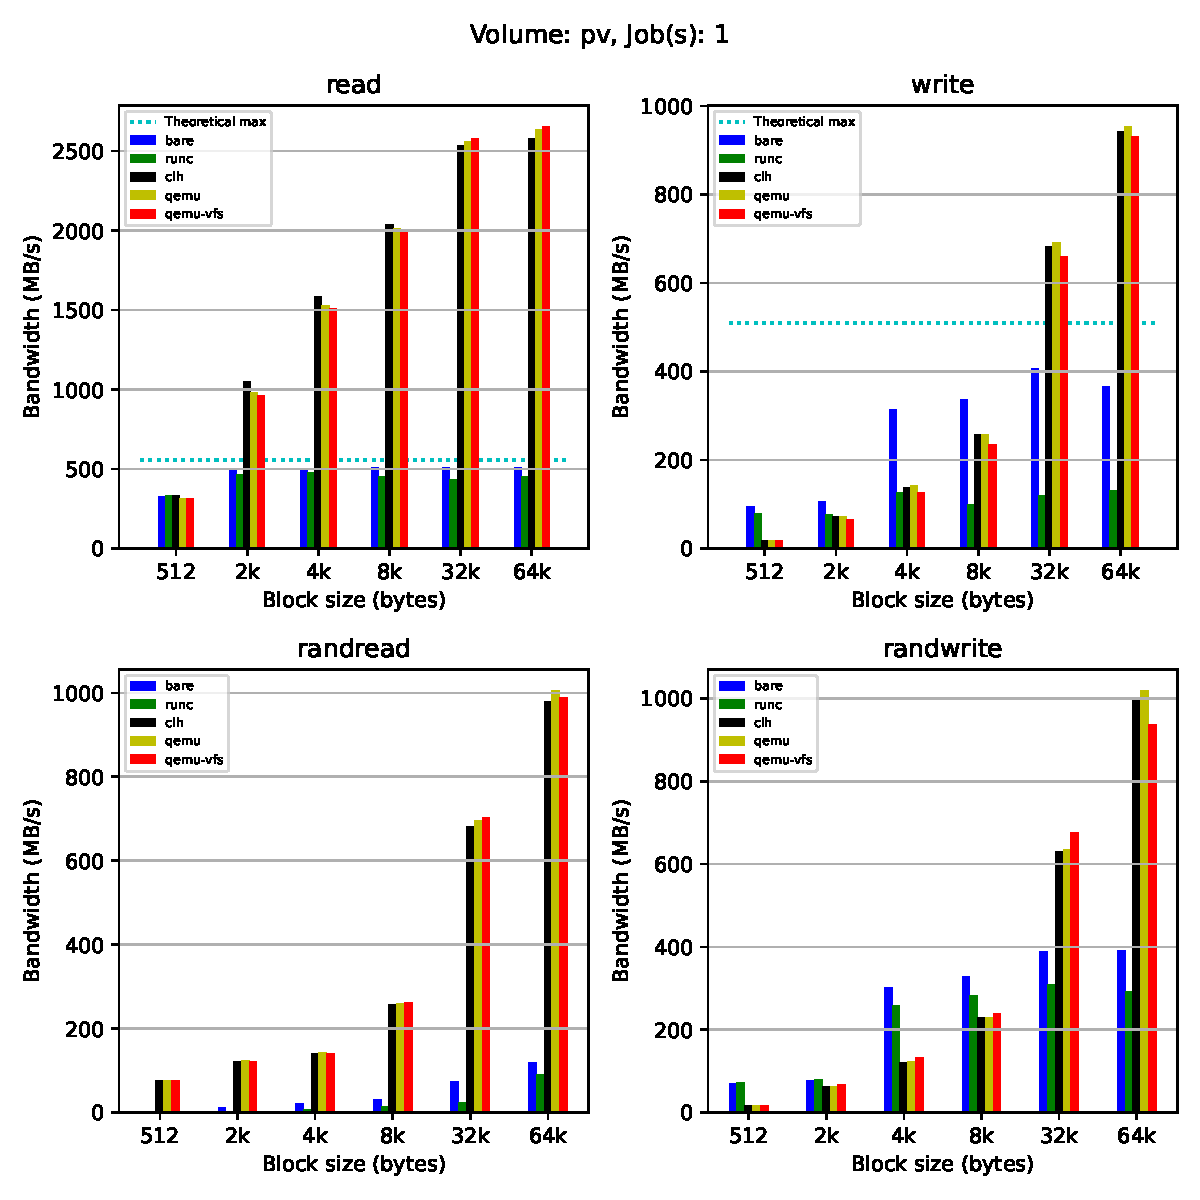
\includegraphics[width=12cm]{results/subplot_bw_by_bs_with_bare(pv,1).pdf}
    \caption{Bandwidth comparison for Persistent Volume by block sizes for all runtime classes with one job}
    \label{fig:ResultsPVByBS-1}
  \end{center}
\end{figure}

Memory-based volume outperforms disk-based storage volumes for two reasons. First, the bandwidth of memory is significantly higher due to architectural differences. Meanwhile, the latency of operations drops close to real-time. Memory-based emptyDir volume is at most 50\% of the memory assigned to the VM \cite{VolumesKubernetes}. The VMs are assigned with 16 GB of memory; thus, the memory-based emptyDir allows at most 8 GB volume. This storage allocation is slightly smaller concerning disk-based storage mediums ED disk and PV. Test environments orchestrated by Kubernetes are launched with a Persistent Volume Claim of 10 GBs. In contrast, bare-metal read operations use the whole 100\% span of the 480 GB SSD \cite{IntelSSD} highly dropping the performance as the operations span across a broader range in the SSD. The smaller volume size allows random seeks to hit with higher confidence, thus increasing the bandwidth of random read operations.

\subsection{Completion latency}

Figures \ref{fig:ResultsEDMEMClatByRTC4096-2} and \ref{fig:ResultsHPClatByRTC4096-2} visualize the performance for completion latency for emptyDir on memory and hostPath volumes by all runtime classes with 4096 byte block sizes and two concurrent jobs. The plots include latencies for 50th and 99th percentile completion of the tasks. RunC narrowly outperforms VM-based runtime classes in memory-based emptyDir by a 3 to 10 ms margin. This tiny difference indicates the overhead from the micro-VM to memory-based operations. The tail for completion of last percentiles in memory-based volume operations is relatively small compared to disk-based emptyDir. Figure \ref{fig:ResultsHPClatByRTC4096-2} includes also bare-metal for comparison in hostPath volume. Overall, bare-metal and runC performs the best with the lowest latencies. Read operations are skewed in favor of micro-VMs due to the caching. Surprisingly, the tail for bare-metal and runC grows along with the last five percentiles in reading operations.

Write operations are less affected by the caching and can be more reliably compared. Bare-metal and runC perform with highly similar results with 4 kB block size and hostPath volume. In Figure \ref{fig:ResultsHPClatByRTC4096-2} the first sequential write task is completed with around 17-19 ms overhead, and the 50th percentile stands at 18-24 ms. RunC adds only 2 ms or 7-8.5\% increment to the bare-metal benchmark for the 99th percentile. Respectively, Kata Containers' runtimes complete the first task at around 200 ms. 50th and 99th percentile are completed at 218-231 ms and 258-272 ms, which is over 200 ms addition.

\begin{figure}[ht]
  \begin{center}
    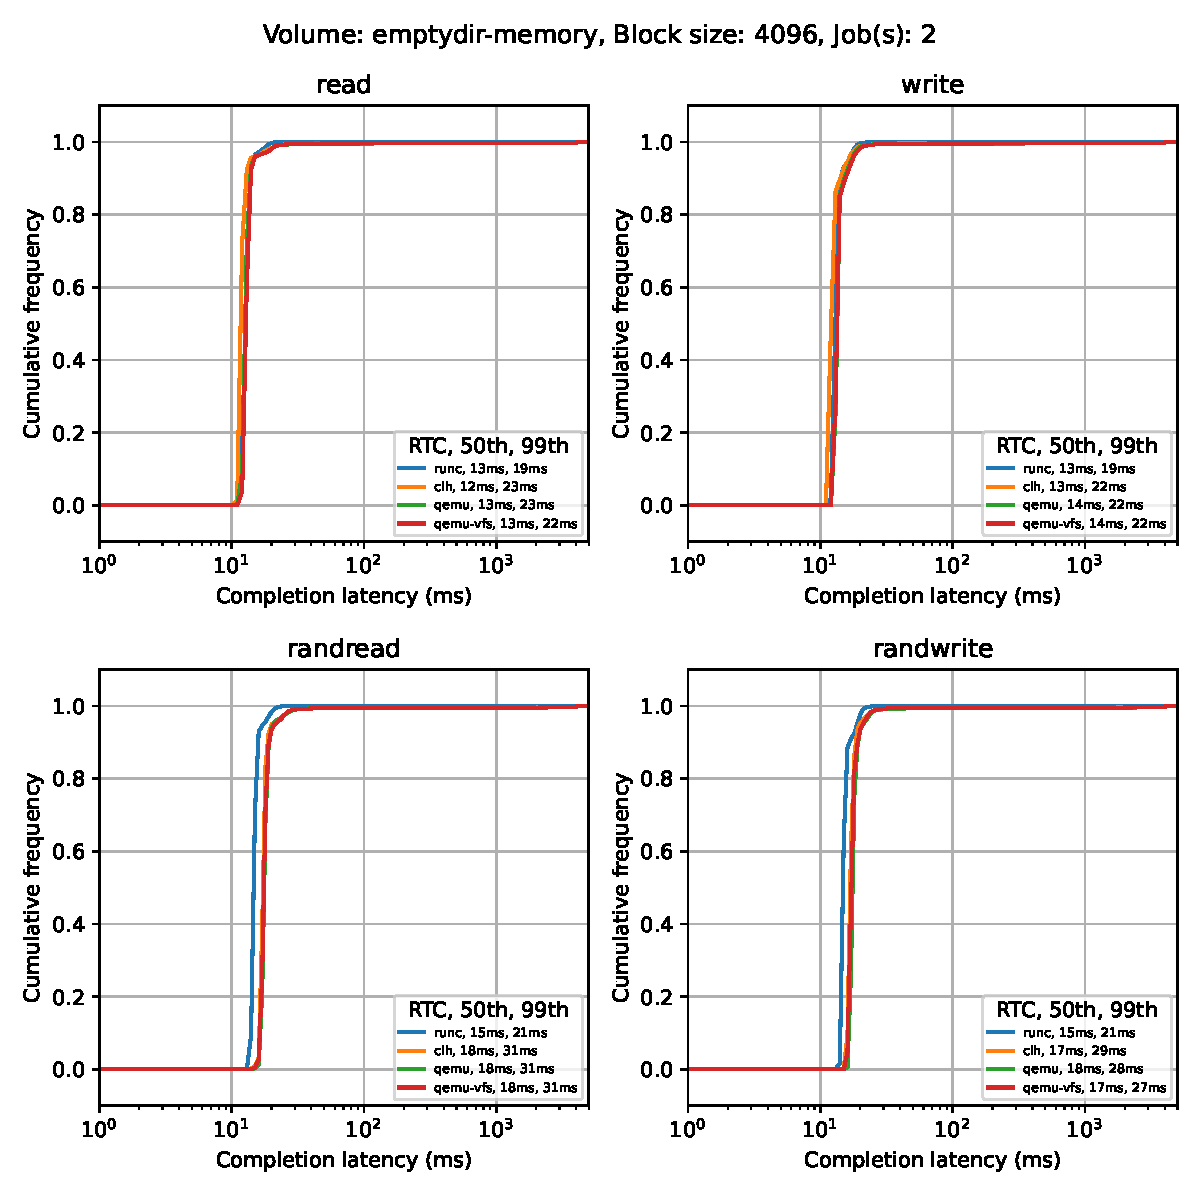
\includegraphics[width=12cm]{results/subplot_clat_bw_by_rw(emptydir-memory,2,4096).pdf}
    \caption{Completion latency for memory-based emptyDir by runtime classes for 4096 bytes block size and two jobs}
    \label{fig:ResultsEDMEMClatByRTC4096-2}
  \end{center}
\end{figure}

\begin{figure}[ht]
  \begin{center}
    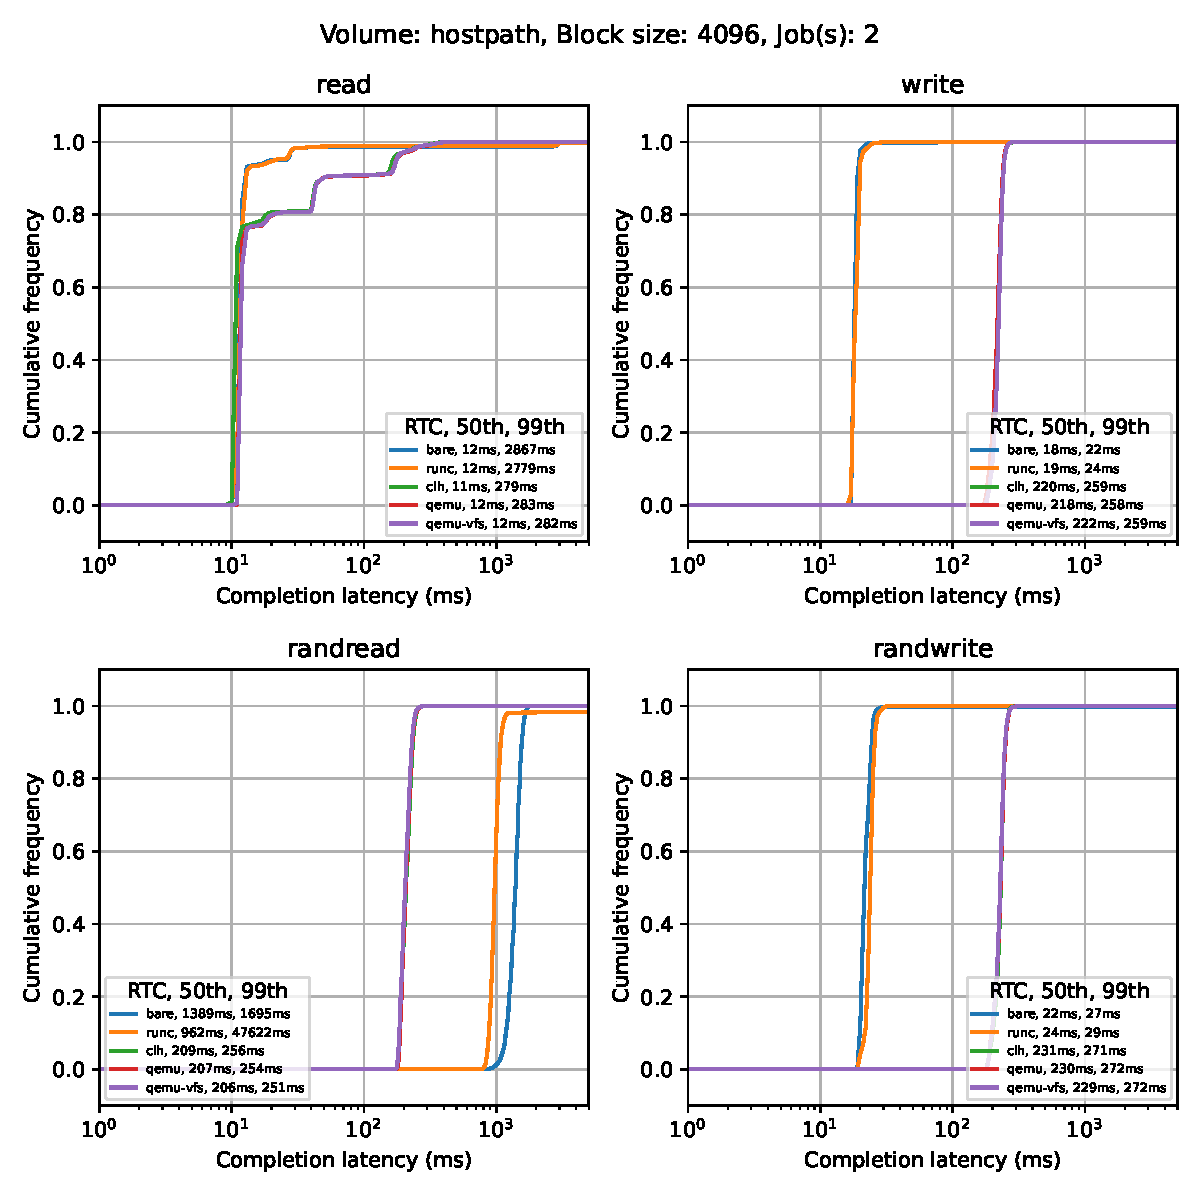
\includegraphics[width=12cm]{results/subplot_clat_bw_by_rw(hostpath,2,4096).pdf}
    \caption{Completion latency for hostPath by runtime classes for 4096 bytes block size and two jobs}
    \label{fig:ResultsHPClatByRTC4096-2}
  \end{center}
\end{figure}

\section{Evaluation}

Caching of the hypervisor significantly affects the received performance results and limits the absolute measurement of the micro-VM's overhead. However, some objections can be derived from the acquired results with confidence. Firstly, Kata Containers acquires close to runC's performance with memory-based emptyDir I/O operations with approximately an 8\% increase in completion latency for 4 kB block size. 

Kata Containers adds overhead to bandwidth and latency to task completion for disk-based operations. In these write operations, the bandwidth overhead is approximately 33-40\% in comparison to runC. For hostPath, the added latency averages around 250 ms even for the first percentile to complete. The architecture of Kata Containers includes a constant delay for the tasks, which stems from the data passing through more components, such as kata-agent and the hypervisor. In contrast, runC relies on a more simple environment allowing instant data transmission. A similar performance trend follows in other disk-based volumes.

The block size of the performance test also affects the results. For smaller block sizes between 512 and 8192, CLH outperforms QEMU-based runtime classes. However, the trend flips for the largest two block sizes in favor of QEMU and QEMU with VirtioFS.

%\textcolor{red}{Transition to Discussion missing?}
 
\chapter{Discussion}
\label{chapter:discussion}

How was the performance? \\
What should be improved? \\
Any gaps in the features or new features for telco environment? \\

\section{Future work}

CPU isolation
Test I/O performance between pods


\section{Conclusion}

% Load the bibliographic references
% ------------------------------------------------------------------
% You can use several .bib files:
% \bibliography{thesis_sources,ietf_sources}
\bibliography{sources}

\appendix
\chapter{Fio jobfile}
\label{appendix:fio_jobfile}

\begin{lstlisting}
[global]
fallocate=none
; Limit runtime
runtime=30
; Jobs run for a specified time limit, not I/O quantity
time_based=1
ioengine=libaio
; Number of I/O units to keep in flight against the file
iodepth=1
direct=0
buffered=1
invalidate=1
ramp_time=0
; Set a number of workers on this client
thread=0
; NUM_JOBS options 1, 2, and 3
numjobs=${NUM_JOBS}
group_reporting=1
; Each file for each job thread is this size
filesize=2G
size=2G
filename_format=$jobnum.dat

[fio-job]
; FIO_RW options read, write, randread, and randwrite
rw=${FIO_RW}
\end{lstlisting}



\end{document}
